% !TEX TS-program = pdflatex
% !TEX encoding = UTF-8 Unicode


\documentclass[11pt]{article} % use larger type; default would be 10pt

\usepackage[utf8]{inputenc} % set input encoding (not needed with XeLaTeX)
\usepackage[portuges]{babel}

\newcommand{\myparagraph}[1]{\paragraph{#1}\mbox{}\\}
\setcounter{secnumdepth}{5}
\setcounter{tocdepth}{5}

%%% PAGE DIMENSIONS
\usepackage{a4}

\usepackage{graphicx} % support the \includegraphics command and options
\graphicspath{ {./UI/}{./VPP/}{./UCASES/}{./INTERFACE/}}
%%% PACKAGES
\usepackage{float}
\usepackage{caption}
\usepackage{booktabs} % for much better looking tables
\usepackage{array} % for better arrays (eg matrices) in maths
\usepackage{paralist} % very flexible & customisable lists (eg. enumerate/itemize, etc.)
\usepackage{verbatim} % adds environment for commenting out blocks of text & for better verbatim
\usepackage{subfig} % make it possible to include more than one captioned figure/table in a single float
% These packages are all incorporated in the memoir class to one degree or another...

\usepackage{xcolor}
\usepackage{rotating}

\setcounter{secnumdepth}{5}

%%% HEADERS & FOOTERS
\usepackage{fancyhdr} % This should be set AFTER setting up the page geometry
\pagestyle{fancy} % options: empty , plain , fancy
\renewcommand{\headrulewidth}{0pt} % customise the layout...
\lhead{}\chead{}\rhead{}
\lfoot{}\cfoot{\thepage}\rfoot{}

%%% SECTION TITLE APPEARANCE
\usepackage{sectsty}
\allsectionsfont{\sffamily\mdseries\upshape} % (See the fntguide.pdf for font help)
% (This matches ConTeXt defaults)

%%% ToC (table of contents) APPEARANCE
\usepackage[nottoc,notlof,notlot]{tocbibind} % Put the bibliography in the ToC
\usepackage[titles,subfigure]{tocloft} % Alter the style of the Table of Contents
\renewcommand{\cftsecfont}{\rmfamily\mdseries\upshape}
\renewcommand{\cftsecpagefont}{\rmfamily\mdseries\upshape} % No bold!

\begin{document}

\begin{titlepage}
\center % Center everything on the page
\newcommand{\HRule}{\rule{\linewidth}{0.4mm}} % Barra horizontal
\textsc{\LARGE Universidade do Minho}\\[0.5cm] % Name of your university/college
\vspace{1cm}
\textsc{\large Mestrado Integrado em Engenharia Informática}\\[1.5cm] % Nome do curso

\includegraphics[scale=0.2]{fotoscap/um.jpg}\\[0.5cm] % Imagem
\vspace{0.5cm}

\HRule \\[1cm]
{ \Huge \bfseries ConfiguraFácil - Relatório}\\[0.7cm] % Título
\HRule \\[1cm]
\vspace{0.1cm}
 
\textsc{\Large \textbf{Desenvolvimento Sistemas Software}}\\[0.75cm] % Nome da UC
\vspace{0.1cm}

%Grupo
\textsc{\large{Grupo 35}}\\[0.8cm]
 
%Autores

\begin{table}[!htbp]
\centering
\begin{tabular}{cc}
 Diogo Sobral (a82523) &  Henrique Pereira (a80261) \\
 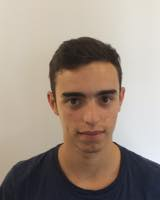
\includegraphics[height=0.8in]{fotoscap/Diogo.jpg} &  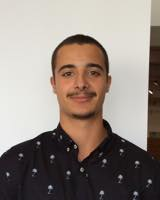
\includegraphics[height=0.8in]{fotoscap/Henrique.jpg} \\
	& \\
 Pedro Moreira (a82364)  &   Pedro Ferreira (a81135) \\
 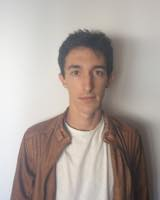
\includegraphics[height=0.8in]{fotoscap/PedroM.jpg} & 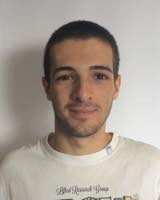
\includegraphics[height=0.8in]{fotoscap/PedroF.jpg} \\

\end{tabular}
\end{table}

{\large 2018/2019}\\[2cm] % Data

\vfill % Fill the rest of the page with whitespace
\end{titlepage}

\tableofcontents
\newpage

\section{Introdução}
A primeira fase do projeto da UC Desenvolvimento de Sistemas de Software consistiu no desenvolvimento dos modelos de domínio, use cases e da interface com o utilizador para a aplicação ConfiguraFácil. 

Na segunda fase, desenvolvemos os diagramas de sequência, de pacotes, de implementação e de classes. Além disso, procedemos também a implementação da aplicação em si, utilizando os modelos desenhados previamente. Para tal, utilizamos DAOs para podermos fazer a conexão entre a base de dados e a aplicação em JAVA. Alterámos também alguns modelos que apresentamos na fase anterior, corrigindo para uma versão que mais se foca nos objetivos da aplicação que pretendíamos modelar.

A aplicação \textit{ConfiguraFácil} consiste numa ferramenta existente nos stands de automóveis, que permite junto dos clientes criar uma configuração para uma encomenda de um carro novo. A aplicação guia o cliente em cada fase da configuração, permitindo-lhe escolher componentes individuais ou pacotes pré-definidos. 

Da perspetiva do grupo, a aplicação apresenta os seguintes requisitos:
\begin{itemize}
	\item O cliente pode escolher a pintura, jantes e pneus, motorização e detalhes interiores e exteriores;
	\item O cliente pode também escolher um pacote pré-definido que consiste num agregado de componentes individuais;
	\item Cada componente deve ter uma designação, preço, lista de componentes incompatíveis e lista de componentes complementares;
	\item Sempre que um componente é adicionado à configuração, a aplicação deve verificar se existe alguma incompatibilidade com algum componente previamente selecionado. Se tal existir, o cliente pode optar por desistir da seleção feita ou remover o produto incompatível. Além disso, deve também verificar se é necessário instalar algum componente complementar. Caso aconteça, o cliente pode manter a opção e instalar os componentes necessários ou então desistir da seleção;
	\item Quando um pacote pré-definido é selecionado, devem ser feitas as verificações de dependência/incompatibilidade para cada um dos componentes do pacote;
	\item Deve haver descontos associados aos pacotes, ou seja, os pacotes devem ser mais baratos que a soma os preços individuais de cada um dos seus componentes;
	\item Se o cliente selecionar individualmente todos os componentes que compõem um pacote, a aplicação deve reconhecer tal pacote e aplicar o respetivo desconto;
	\item Após as escolhas básicas, como a pintura e a motorização, o cliente deve poder indicar um orçamento para a encomenda e o sistema deve propor a melhor configuração possível dentro do orçamento apresentado. Ou seja, a aplicação deve conseguir gerar uma configuração ótima dado um orçamento;
	\item Cada componente deve ter um stock associado;
	\item Sempre que chega um novo stock de componentes, o sistema deve conseguir determinar quais são os carros que podem ser produzidos;
	\item Os carros são produzidos por ordem de chegada à fila de configurações efetuadas pelos clientes.
\end{itemize}
Desta forma, procuramos cobrir todos estes requisitos, de forma a que a aplicação seja o mais completa e coesa possível. Além do referido, incluímos também as funcionalidades de registar, identificar, consultar e alterar clientes, login de funcionários (sendo que o administrador pode registar, remover ou alterar os dados destes) e as funcionalidades relativas à gestão de fábrica de registar entrada de stock no sistema e produzir encomendas.

\section{Diagrama de Domínio}
Para a aplicação que nos foi proposta e que descrevemos acima, desenvolvemos o diagrama de domínio que apresentamos de seguida:
\begin{center}
 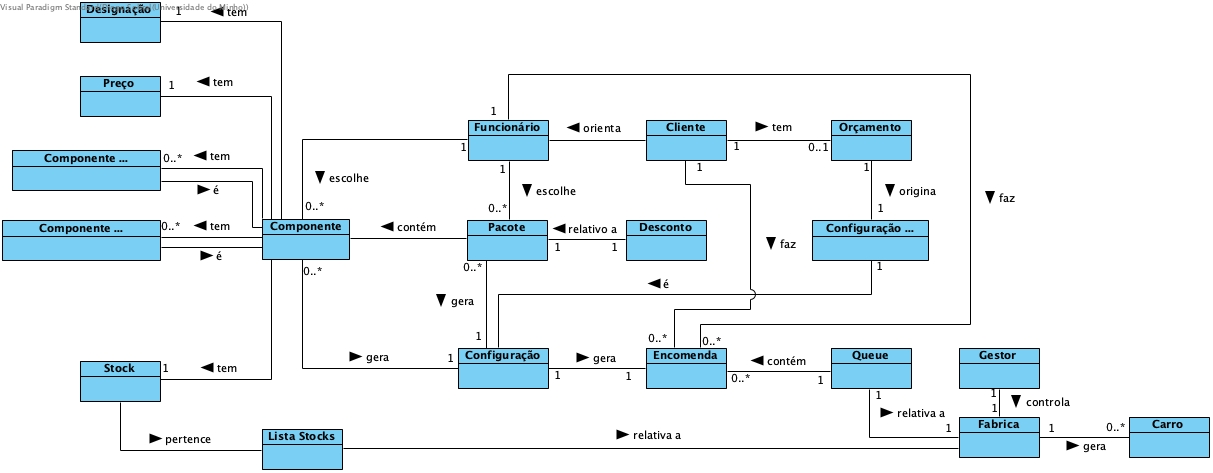
\includegraphics[width = 6.5in]{VPP/Dominio.jpg}
\end{center}

\newpage

%\begin{center}
%\section*{1ª Fase}
%\end{center}

\section{Diagrama de Use Cases}
\label{useCases}
\subsection{Diagramas}
Os Use Cases por nós apresentados e especificados na secção seguinte foram organizados em seis diagramas:

\subsubsection{Geral}
		\begin{center}
 			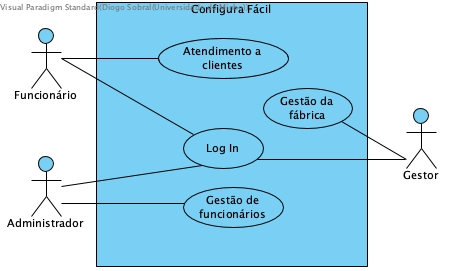
\includegraphics[scale = 0.7]{D_USECASE/Geral.jpg}
		\end{center}
\subsubsection{Gestão de Funcionários}
		\begin{center}
 			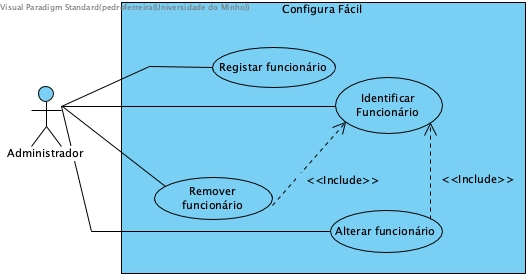
\includegraphics[scale = 0.7]{D_USECASE/Gestao_de_funcionarios.jpg}
		\end{center}\newpage
\subsubsection{Gestão de Clientes}
		\begin{center}
 			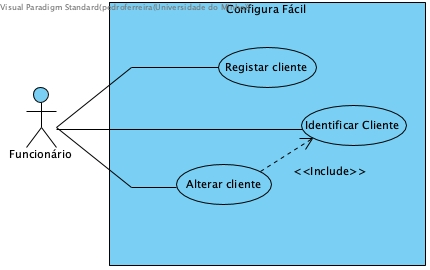
\includegraphics[scale = 0.7]{D_USECASE/Gestao_de_clientes.jpg}
		\end{center}
\subsubsection{Atendimento a Clientes}
		\begin{center}
 			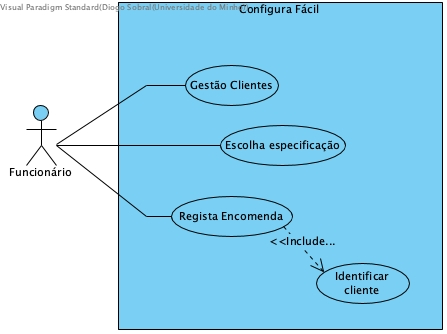
\includegraphics[scale = 0.7]{D_USECASE/Atendimento_a_clientes.jpg}
		\end{center}\newpage
\subsubsection{Escolha da Especificação}
		\begin{center}
 			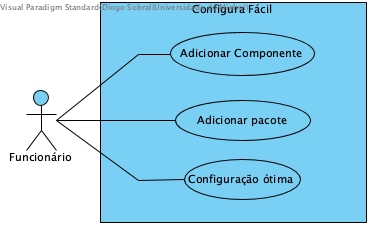
\includegraphics[scale = 0.7]{D_USECASE/Escolha_da_especificacao.jpg}
		\end{center}
\subsubsection{Gestão da Fábrica}
		\begin{center}
 			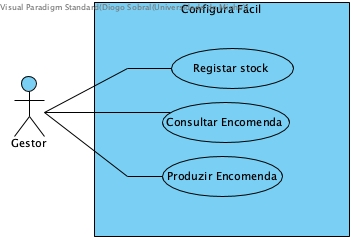
\includegraphics[scale = 0.7]{D_USECASE/Gestao_da_fabrica.jpg}
		\end{center}
\subsection{Atores}
\subsubsection{Funcionário}
Representa um funcionário do stand responsável por atender os clientes. Um funcionário tem permissões para poder gerar configurações e registar encomendas. Cabe a um funcionário a parte de gestão dos clientes.

\subsubsection{Gestor}
Representa um funcionário do stand que trabalha na parte da produção de carros. Este ator é responsável por gerir o stock e encomenda-lo. Um gestor tem acesso a todas as encomendas que ainda não foram produzidas e é este de decide qual destas deve avançar mediante o stock existente.

\subsubsection{Administrador}
Representa a pessoa do stand responsável por gerir os funcionários.

\newpage

\section{Especificação de Use Cases}
Nesta secção vamos expor as tabelas de especificação que fizemos para cada um dos Use Cases presentes nos diagramas da secção \ref{useCases}.

Para melhor organização, decidimos dividir as tabelas em Excel da especificação dos Use Cases em quatro ficheiros: 
\subsection{Geral}
\subsubsection{Use Case - Log in}
\begin{center}
 	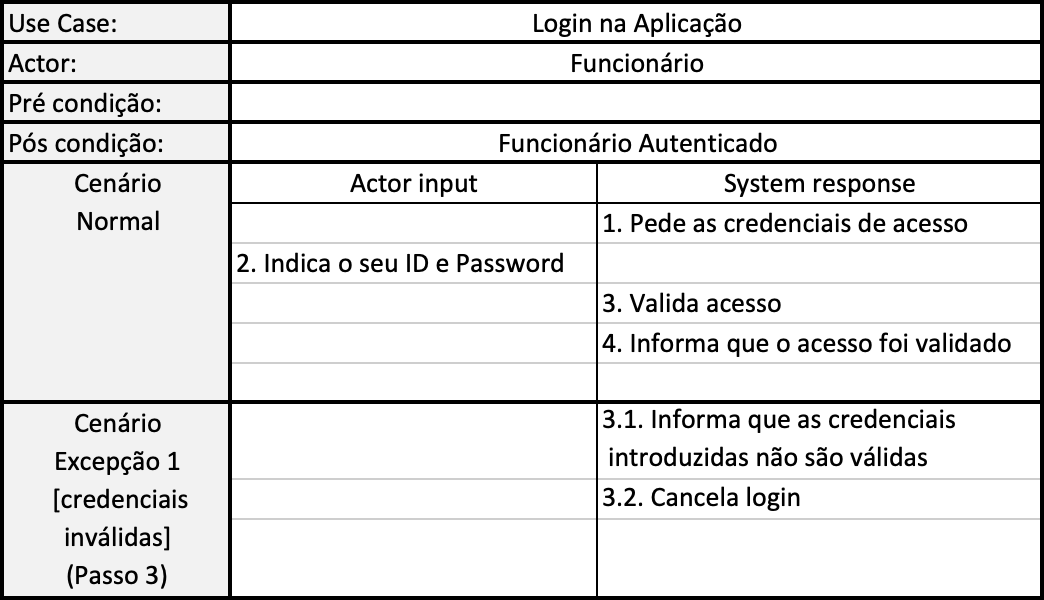
\includegraphics[width = 5.5in]{D_E_USECASE/uc_login.png}
\end{center}
\newpage
\subsection{Gestão de Funcionários}
\subsubsection{Use Case - Identificar Funcionário}
\begin{center}
 	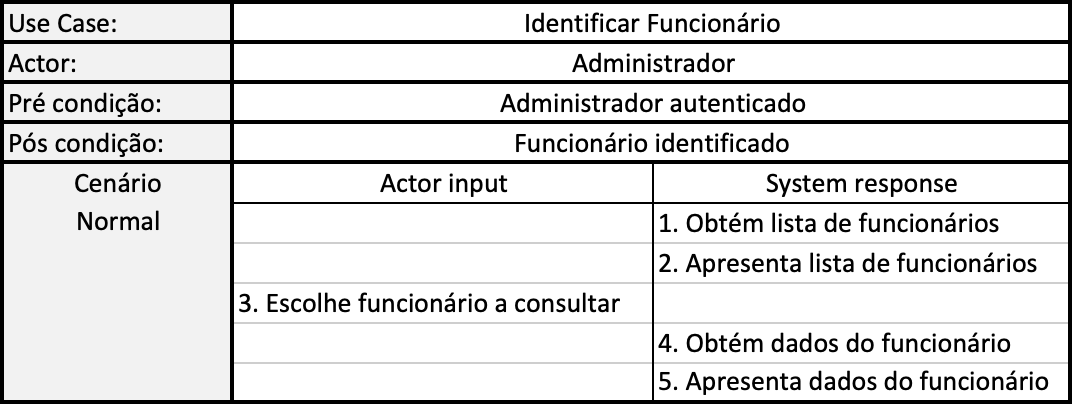
\includegraphics[width = 5.5in]{D_E_USECASE/uc_identificar_funcionario.png}
\end{center}
\subsubsection{Use Case - Registar Funcionário}
\begin{center}
 	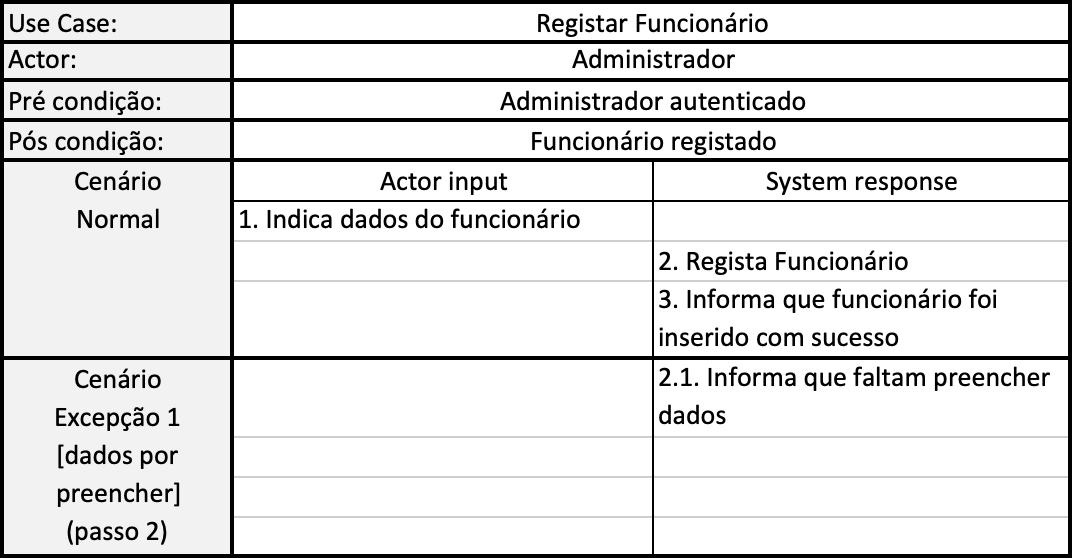
\includegraphics[width = 5.5in]{D_E_USECASE/uc_registar_funcionario.png}
\end{center}
\subsubsection{Use Case - Remover Funcionário}
\begin{center}
 	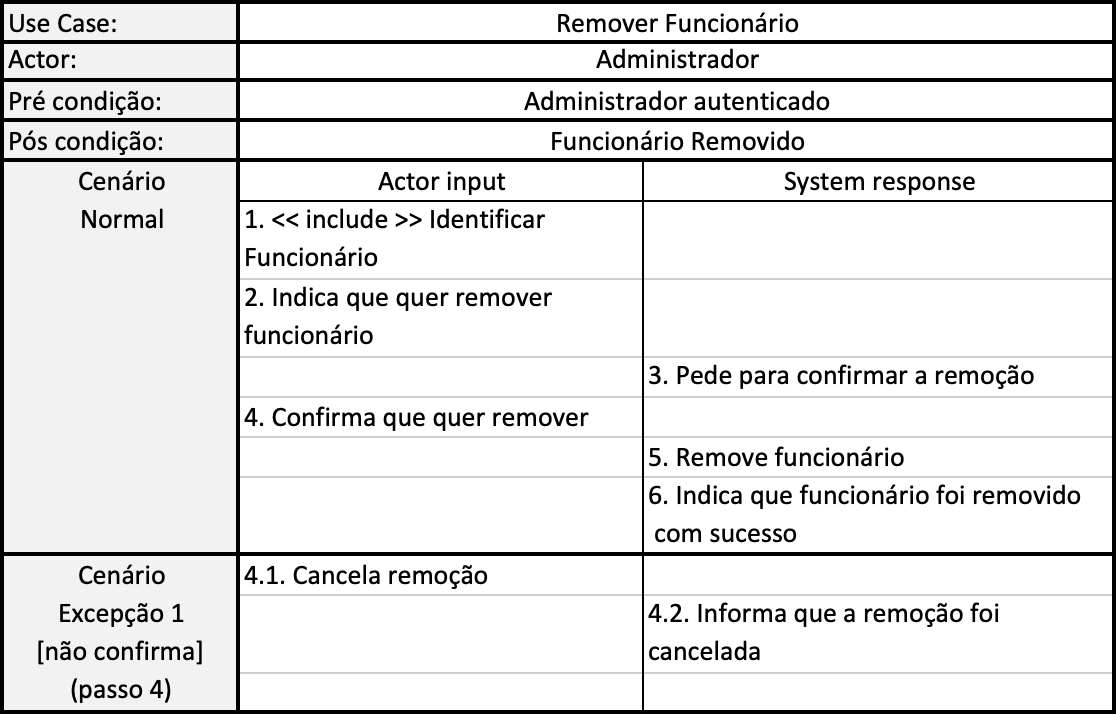
\includegraphics[width = 5.5in]{D_E_USECASE/uc_remover_funcionario.png}
\end{center}
\subsubsection{Use Case - Alterar Funcionário}
\begin{center}
 	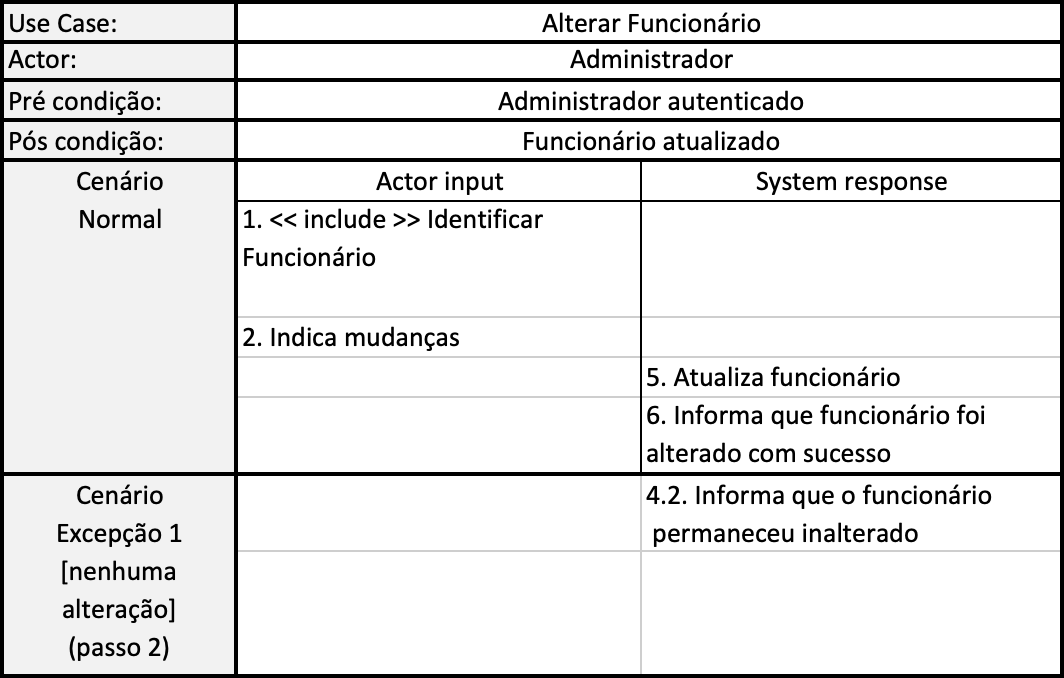
\includegraphics[width = 5.5in]{D_E_USECASE/uc_alterar_funcionario.png}
\end{center}
\subsection{Gestão de Clientes}
\subsubsection{Use Case - Identificar Cliente}
\begin{center}
 	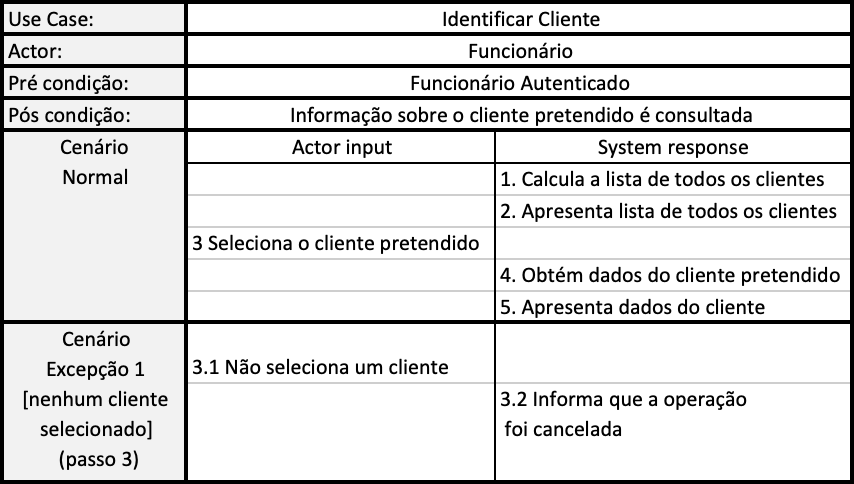
\includegraphics[width = 5.5in]{D_E_USECASE/uc_identificar_cliente.png}
\end{center}
\subsubsection{Use Case - Alterar Cliente}
\begin{center}
 	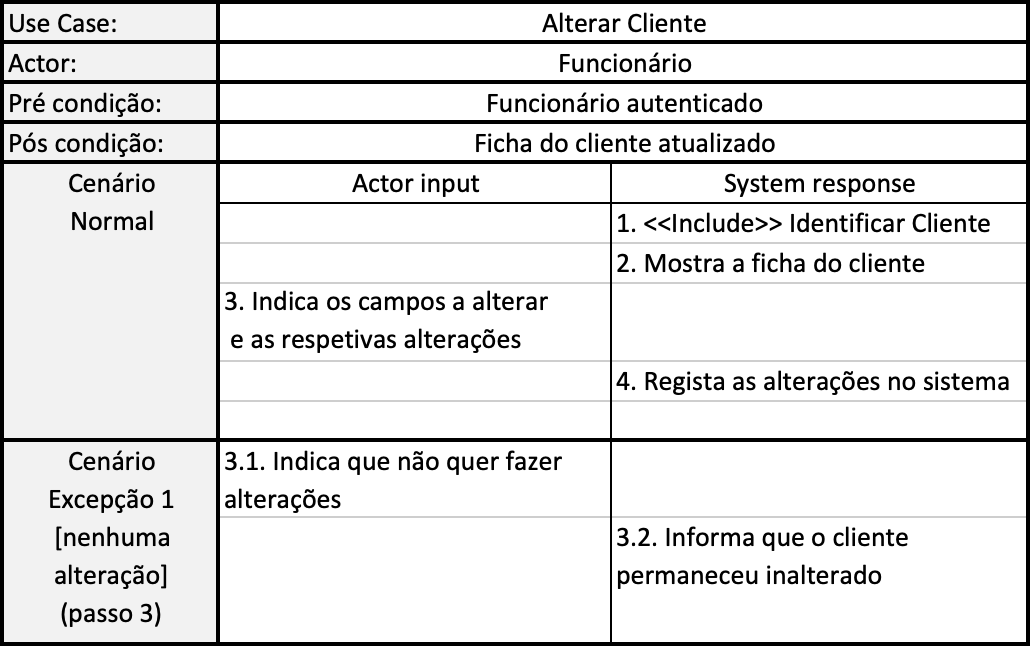
\includegraphics[width = 5.5in]{D_E_USECASE/uc_alterar_cliente.png}
\end{center}
\subsubsection{Use Case - Registar Cliente}
\begin{center}
 	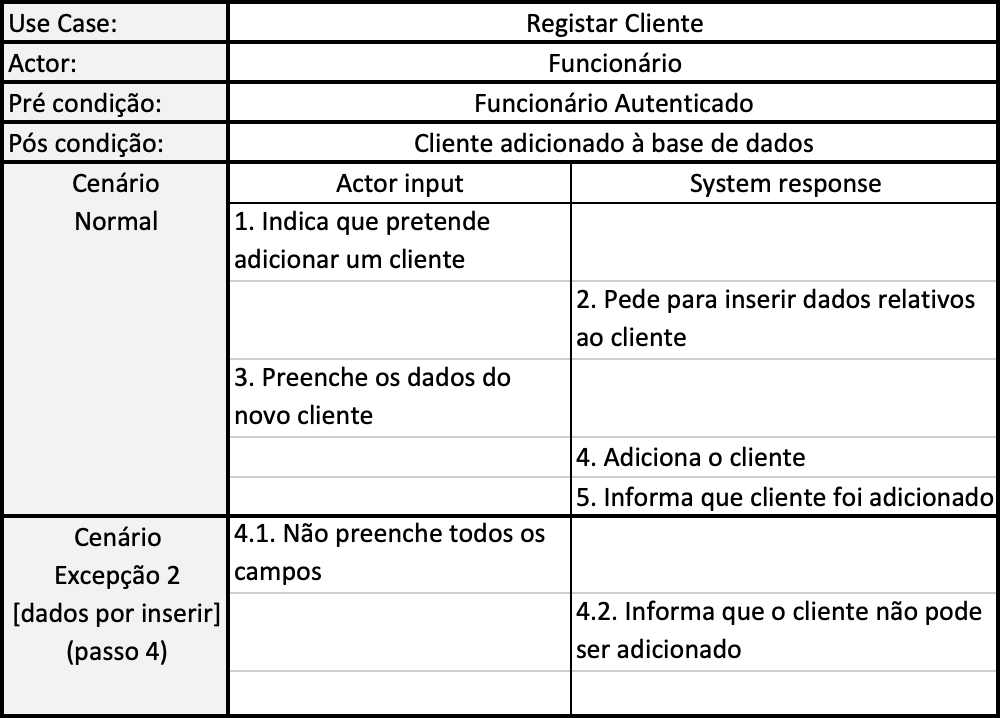
\includegraphics[width = 5.5in]{D_E_USECASE/uc_registar_cliente.png}
\end{center}

\newpage
\subsection{Atendimento a Clientes}
\subsubsection{Use Case - Regista Encomenda}
\begin{center}
 	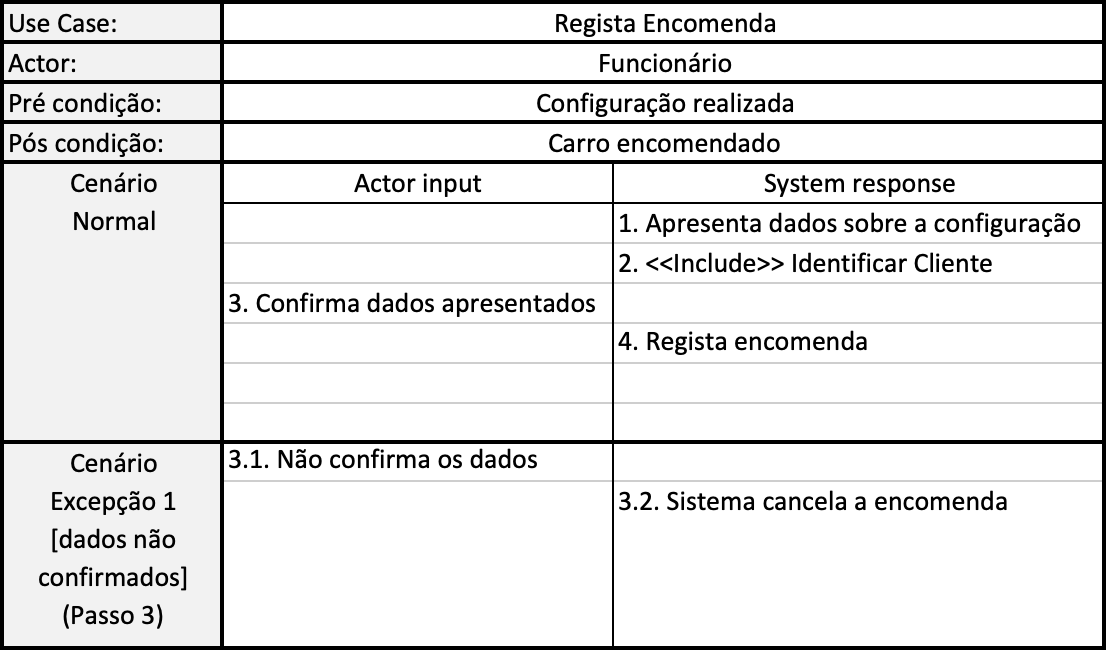
\includegraphics[width = 5.5in]{D_E_USECASE/uc_regista_encomenda.png}
\end{center}

\subsection{Escolha da Especificação}

\subsubsection{Use Case - Adicionar Componente}
\begin{center}
 	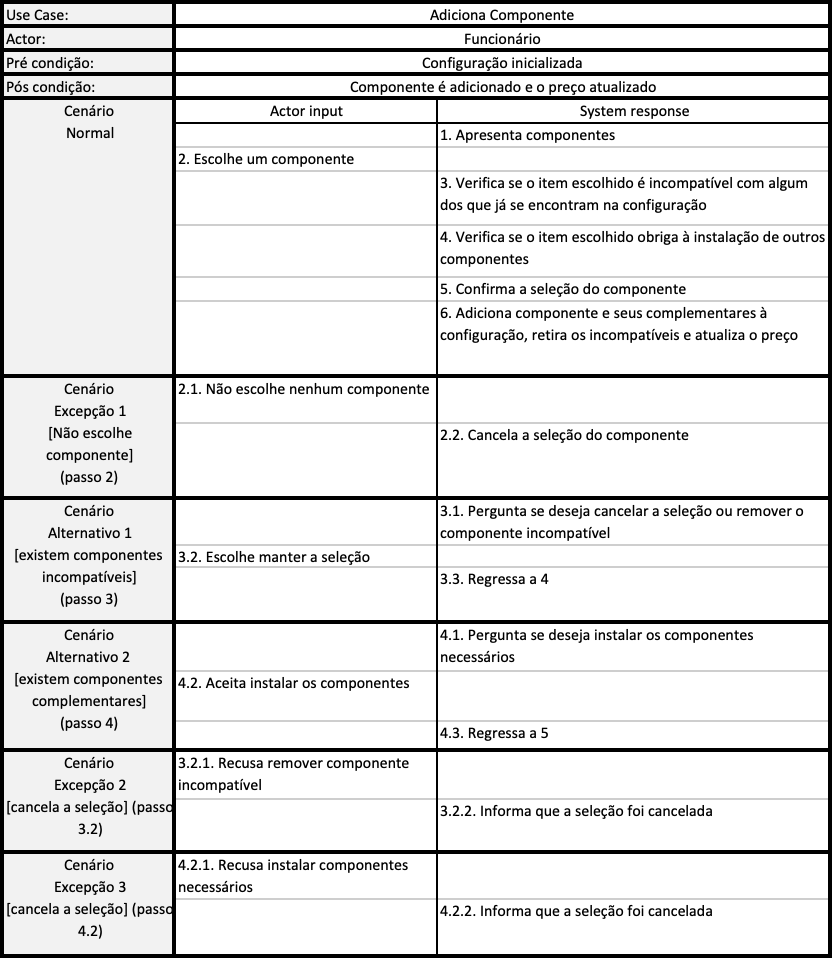
\includegraphics[width = 5.5in]{D_E_USECASE/uc_adiciona_componente.png}
\end{center}
\subsubsection{Use Case - Adicionar pacote}
\begin{center}
 	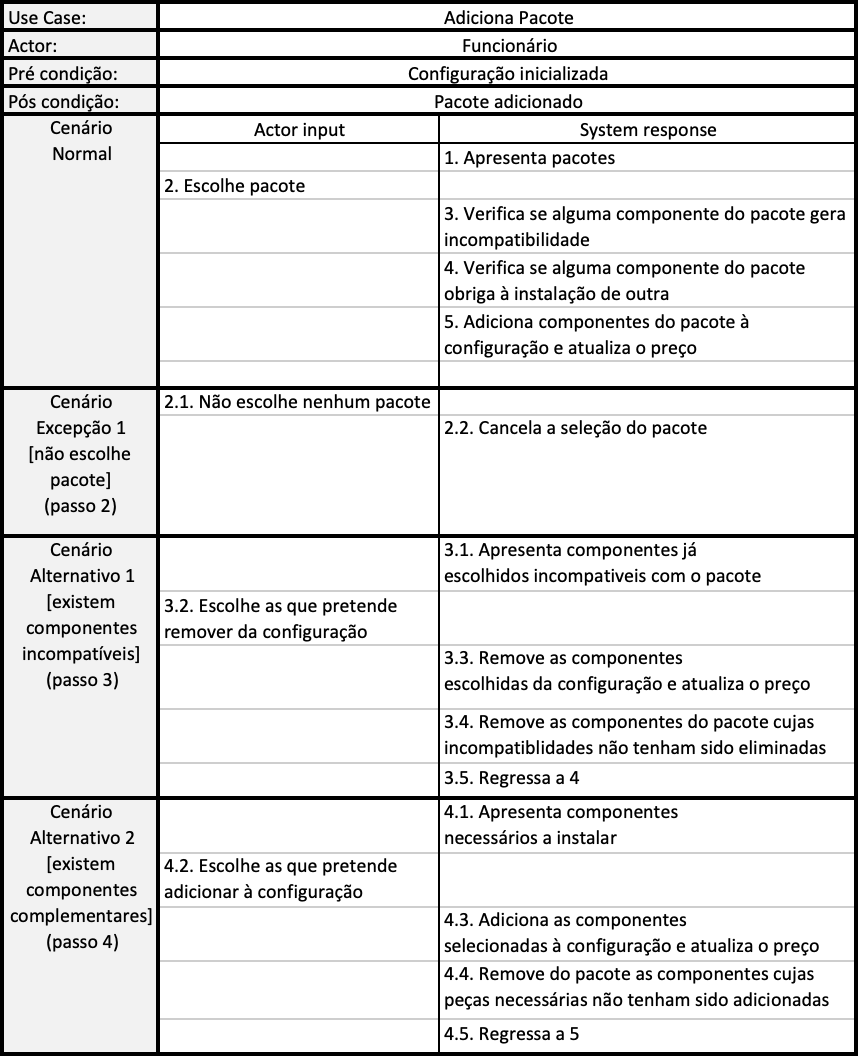
\includegraphics[width = 5.5in]{D_E_USECASE/uc_adicionar_pacote.png}
\end{center}
\subsubsection{Use Case - Configuração Ótima}
\begin{center}
 	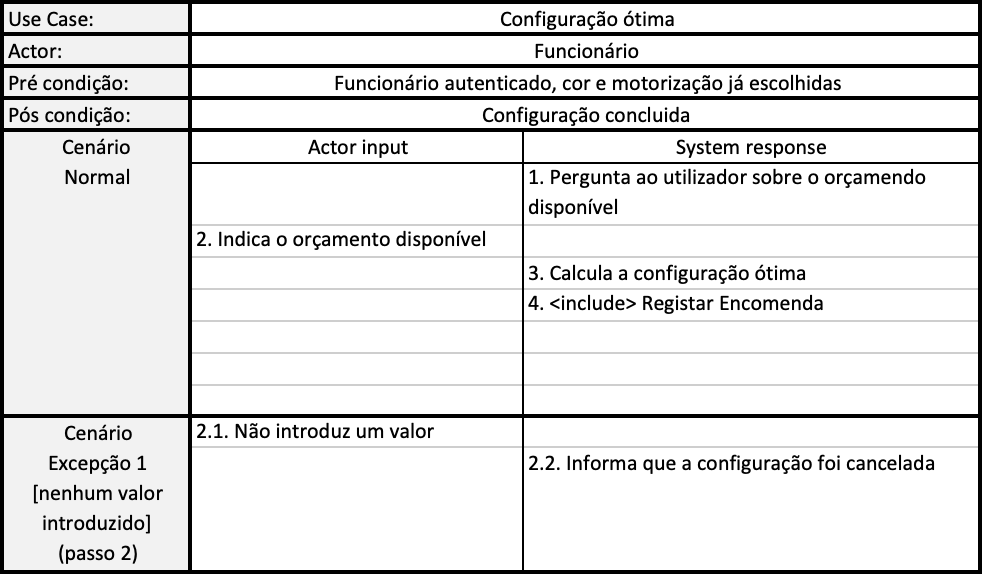
\includegraphics[width = 5.5in]{D_E_USECASE/uc_configuracao_otima.png}
\end{center}

\subsection{Gestão da Fábrica}
\subsubsection{Use Case - Registar Stock}
\begin{center}
 	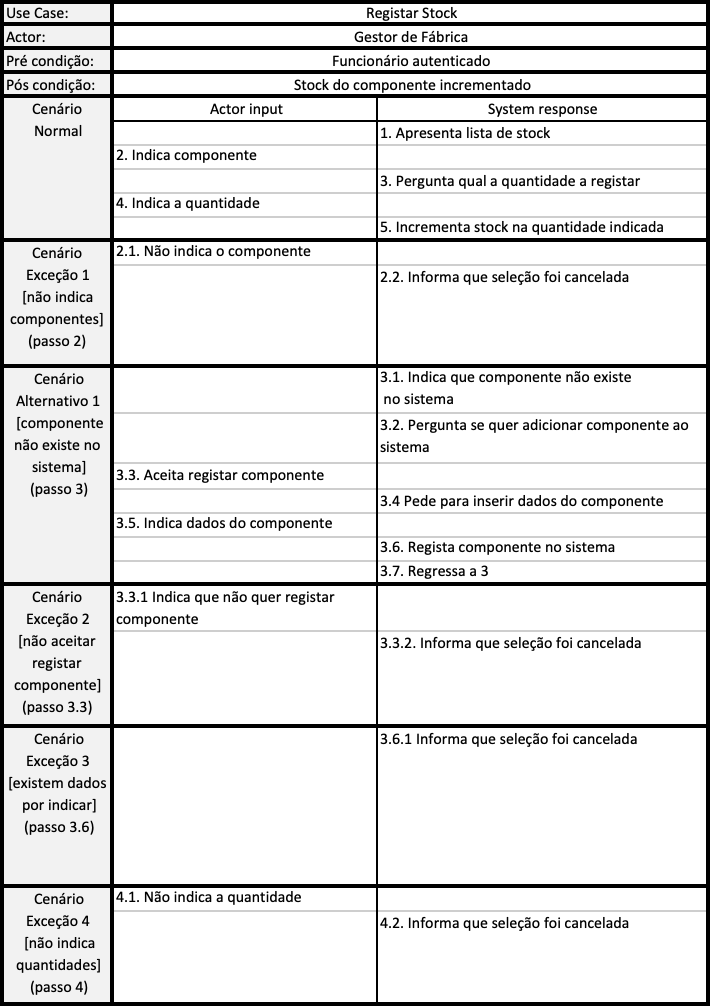
\includegraphics[width = 5.5in]{D_E_USECASE/uc_registar_stock.png}
\end{center}
\subsubsection{Use Case - Consultar Encomenda}
\begin{center}
 	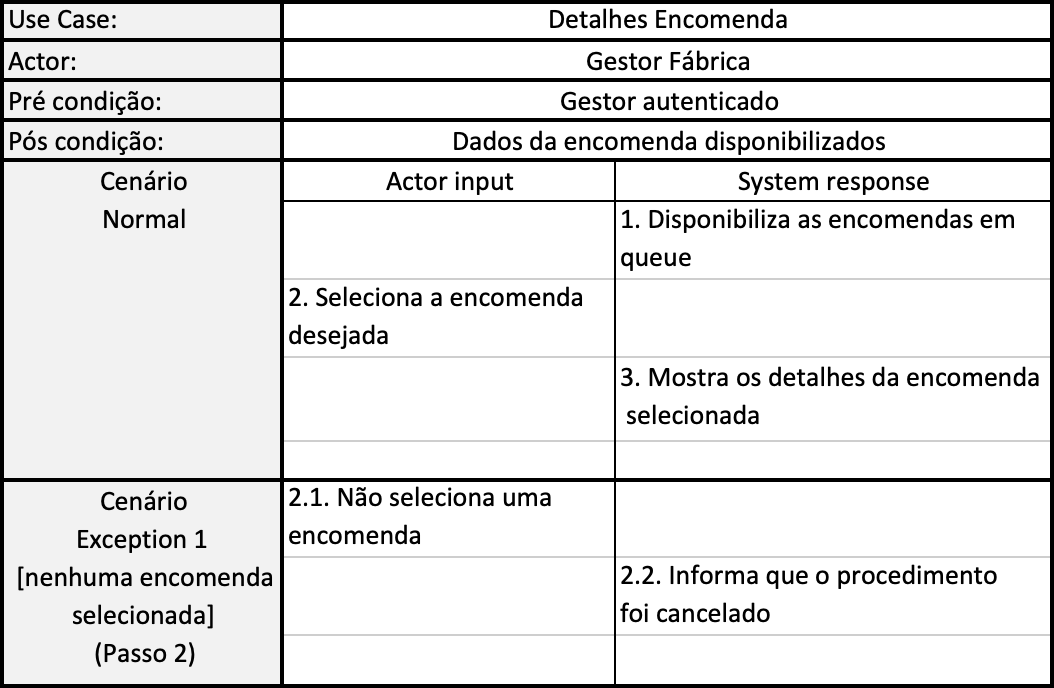
\includegraphics[width = 5.5in]{D_E_USECASE/uc_consultar_encomenda.png}
\end{center}
\subsubsection{Use Case - Produzir Encomenda}
\begin{center}
 	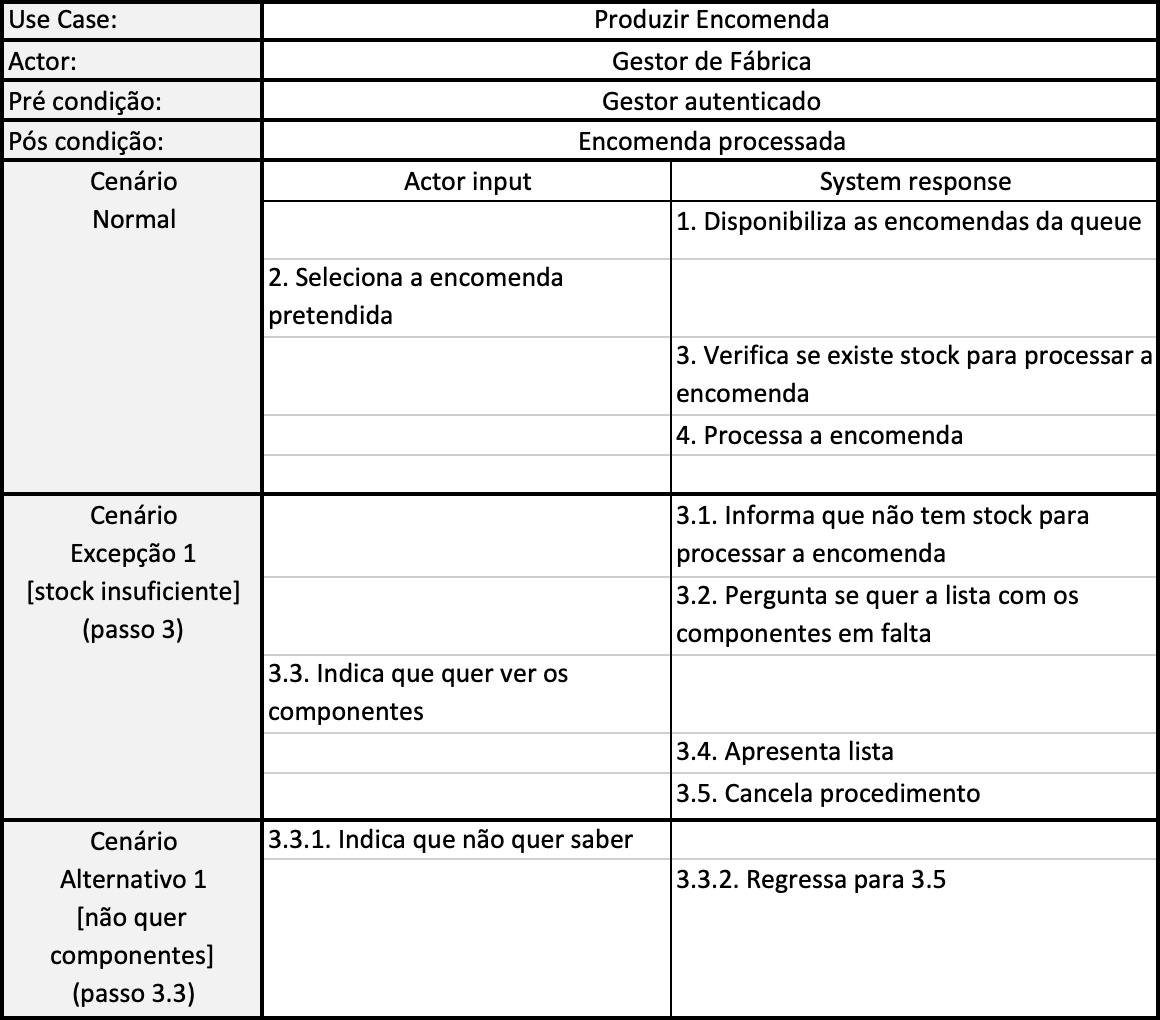
\includegraphics[width = 5.5in]{D_E_USECASE/uc_processar_encomenda.png}
\end{center}
\newpage

\section{Protótipo de Interface}
O protótipo de interface para a aplicação foi feito com o \textit{Pencil}, ferramenta aconselhada pelos docentes da UC.

A página inicial do programa é a pagina de login.
\begin{center}
 	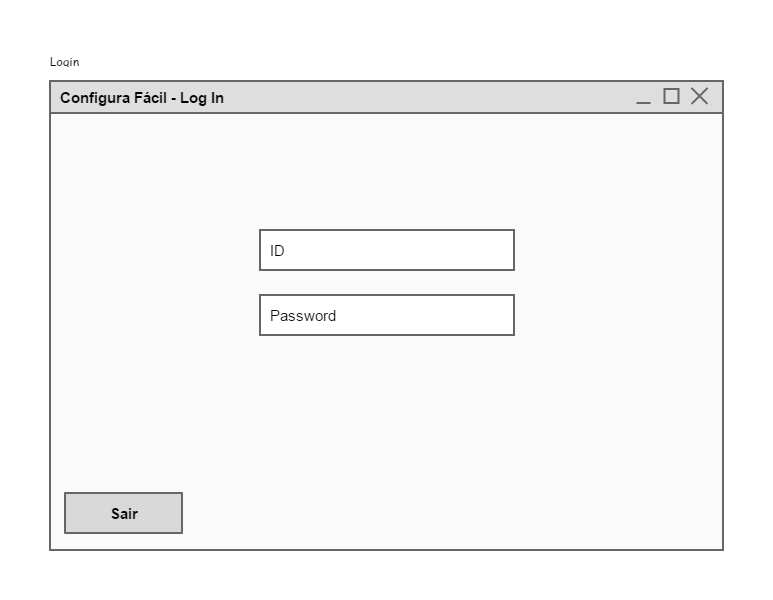
\includegraphics[width = 5in]{Prototipagem/configura_fcil_root.png}
\end{center}

Daqui, o utilizador pode ir para uma das seguintes janelas, dependendo do seu estatuto na aplicação:

\begin{center}
 	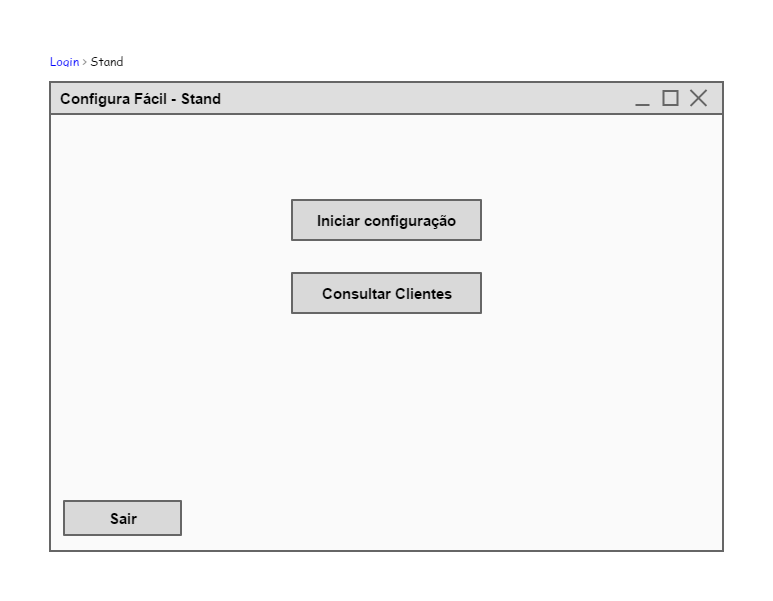
\includegraphics[width = 5.5in]{Prototipagem/configura_fcil_stand.png}

 	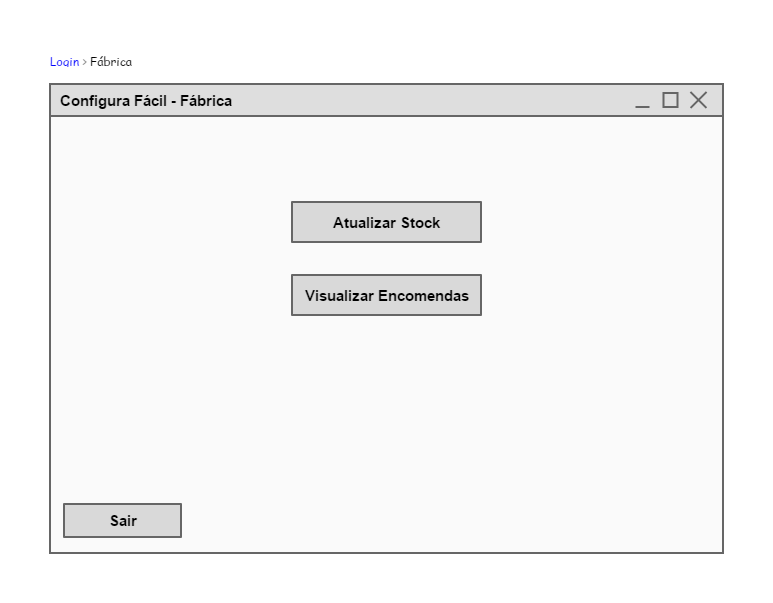
\includegraphics[width = 5.5in]{Prototipagem/configura_fcil_fbrica.png}

 	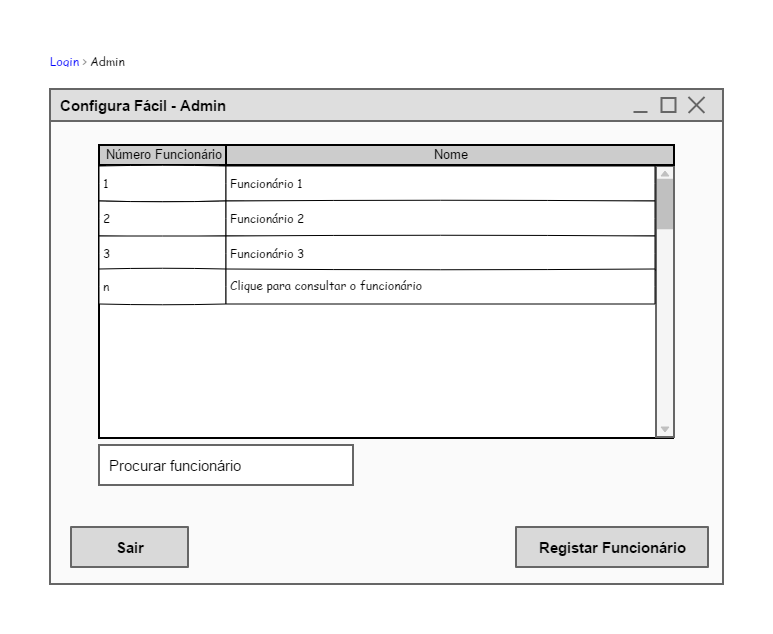
\includegraphics[width = 5.5in]{Prototipagem/configura_fcil_admin.png}
\end{center}


A partir da janela do Stand encontramos a seguinte interface:
\begin{center}
 	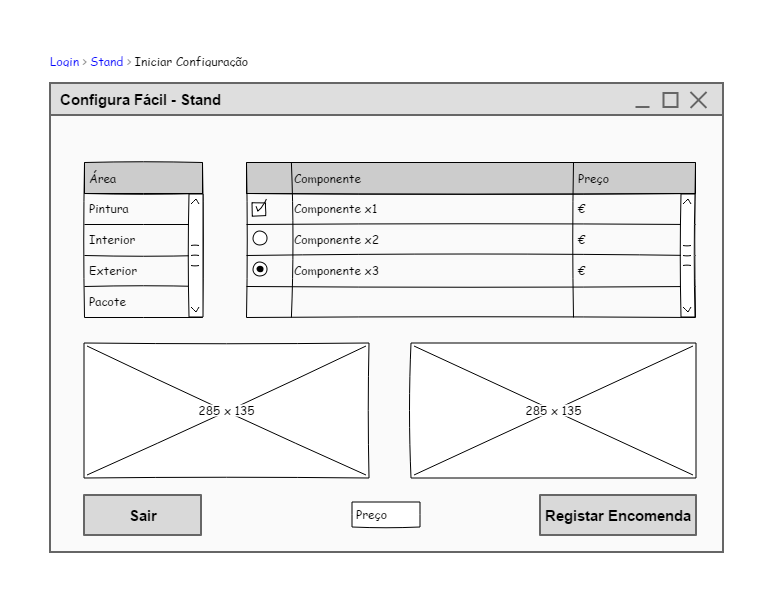
\includegraphics[width = 5in]{Prototipagem/configurao_de_carro.png}

 	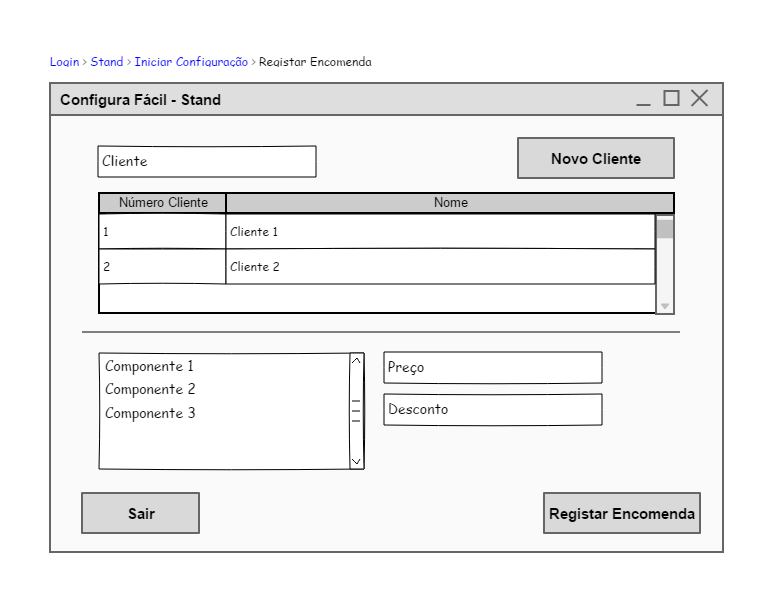
\includegraphics[width = 5.5in]{Prototipagem/registar_encomenda.png}

 	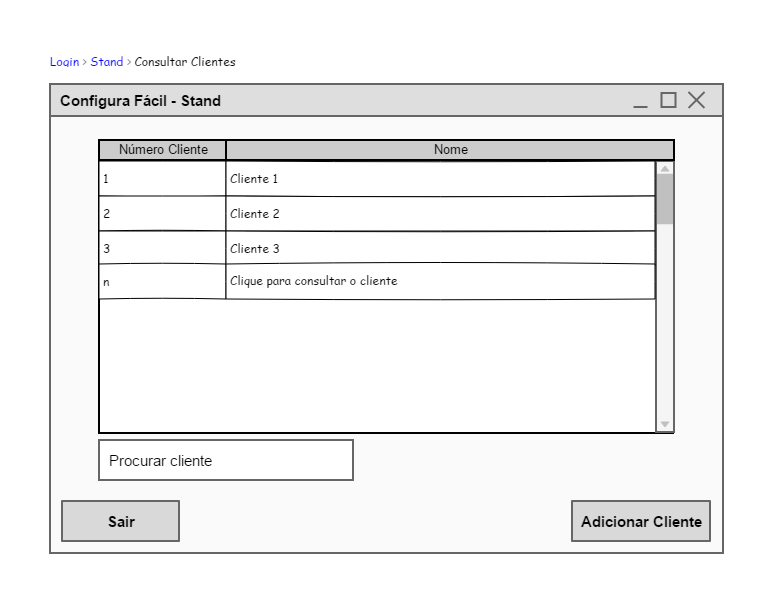
\includegraphics[width = 5.5in]{Prototipagem/consultar_clientes.png}
	
	\begin{table}[]
		\begin{tabular}{cc}
 			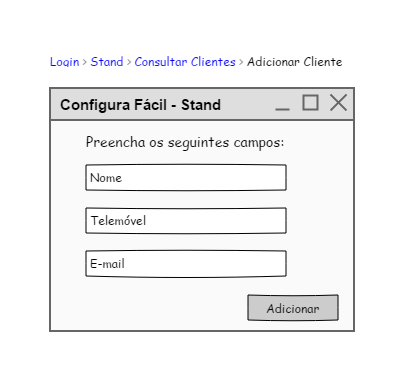
\includegraphics[width = 3in]{Prototipagem/adicionar_cliente.png}	& 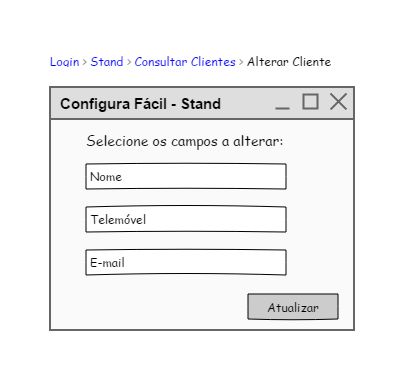
\includegraphics[width = 3in]{Prototipagem/alterar_cliente.png}
		\end{tabular}
	\end{table}
 	 	
\end{center}

Já quando o utilizador é um gestor da fábrica, a interface gráfica que o guiará pela aplicação é a seguinte:
\begin{center}
	\begin{table}[!htbp]
		\begin{tabular}{cc}
 			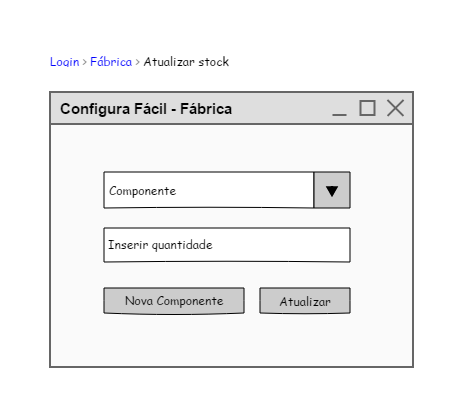
\includegraphics[width = 3in]{Prototipagem/atualizar_stock.png} & 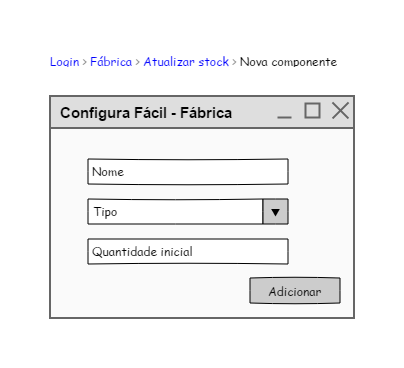
\includegraphics[width = 3in]{Prototipagem/nova_componente.png}
		\end{tabular}
	\end{table}

 	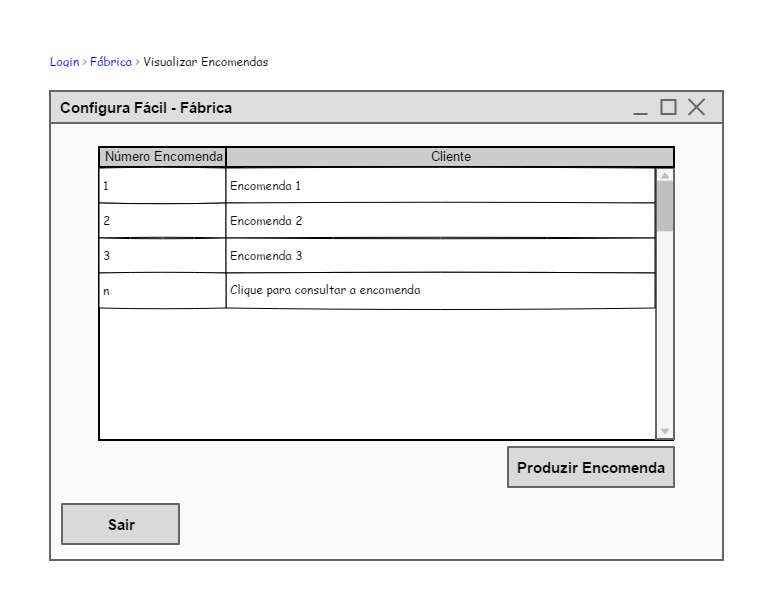
\includegraphics[width = 5.5in]{Prototipagem/visualizar_encomendas.png}

\end{center}

Por fim, quando o funcionário faz o Login como Admistrador será esta a sua visão da aplicação:
\begin{center}
	\begin{table}[!htbp]
		\begin{tabular}{cc}
 			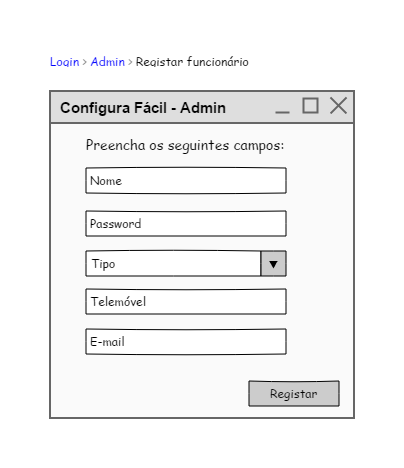
\includegraphics[width = 3in]{Prototipagem/registar_funcionrio.png} & 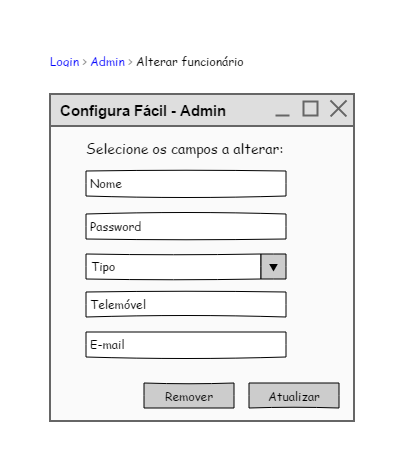
\includegraphics[width = 3in]{Prototipagem/alterar_funcionrio.png}
		\end{tabular}
	\end{table}

\end{center}

\section{Diagrama de Máquinas de Estado}
O diagrama de Máquinas de Estado relativo à interface do programa é o seguinte:
	\begin{center}
		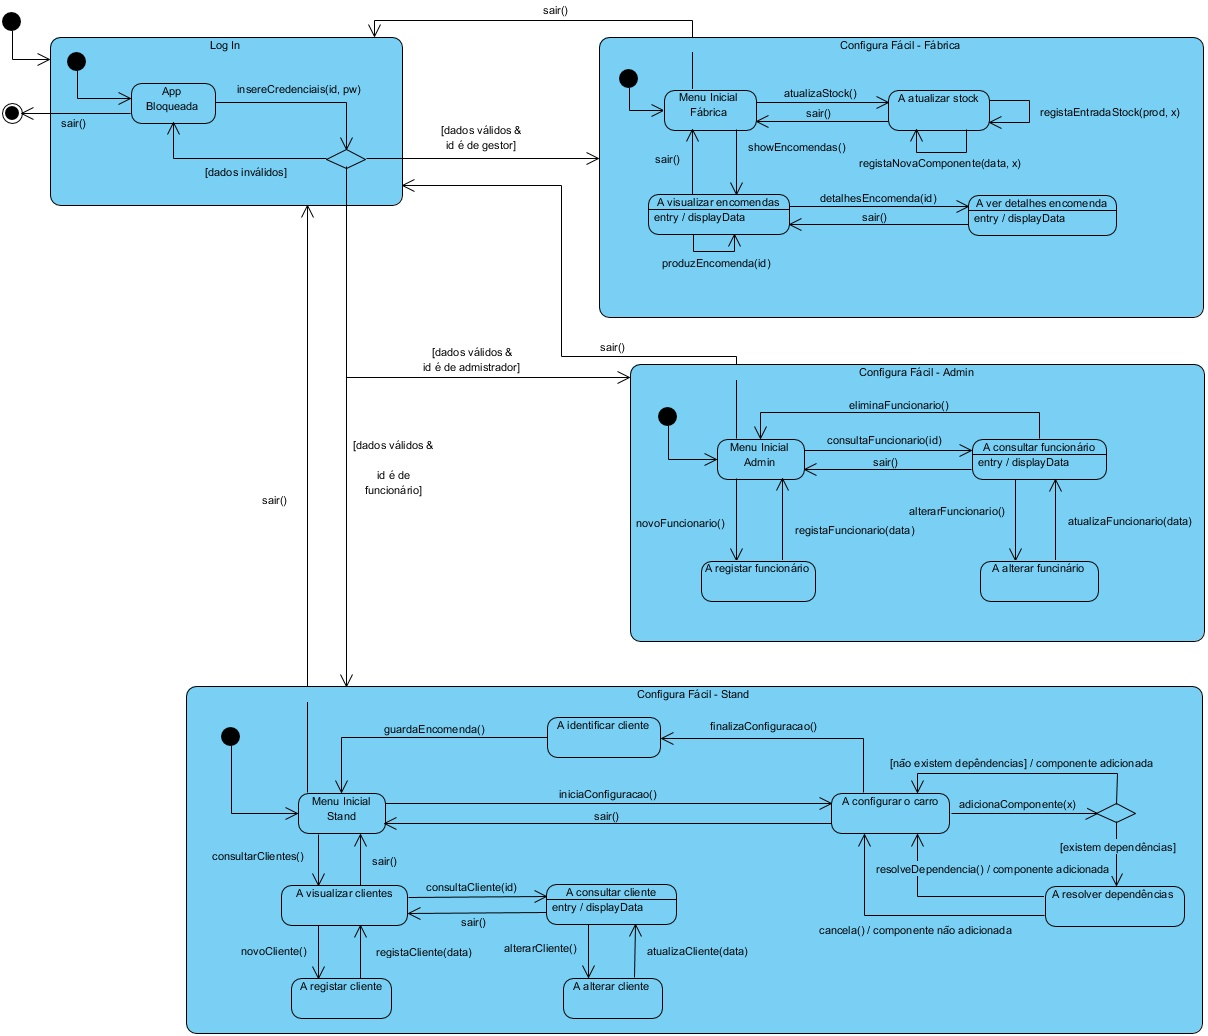
\includegraphics[width = 6in]{VPP/Maquina_de_Estado.jpg}
	\end{center}
\newpage

\section{Diagramas de Sequência de Sistema}
A segunda fase do projeto principiou com a modelação dos diagramas de sequência, partindo da especificação dos Use Cases feita na fase anterior. Assim sendo, temos os seguintes diagramas:

\subsection{Log in}
\begin{center}
 	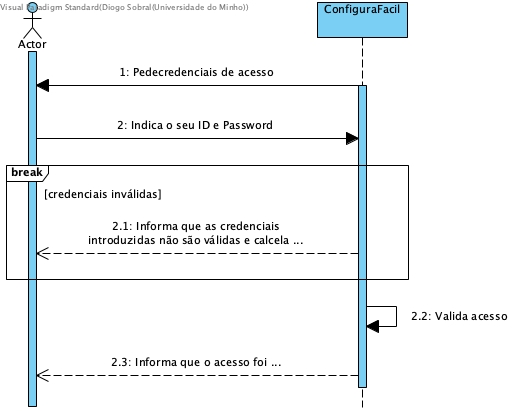
\includegraphics[width = 5.5in]{DSS/DSS-Log_In.jpg}
\end{center}

\subsection{Identificar Funcionário}
\begin{center}
 	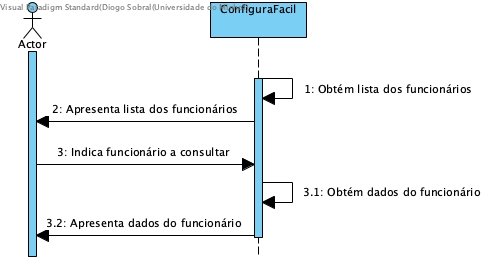
\includegraphics[width = 5.5in]{DSS/DSS-Identificar_Funcionario.jpg}
\end{center}

\subsection{Registar Funcionário}
\begin{center}
 	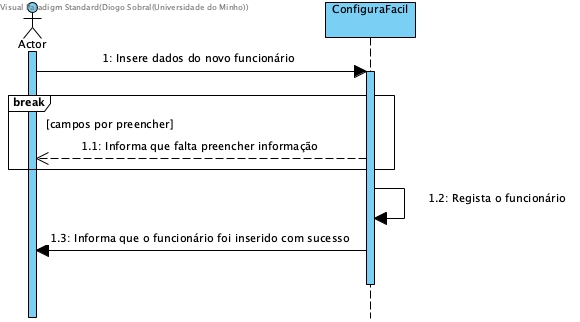
\includegraphics[width = 5.5in]{DSS/DSS-Registar_funcionario.jpg}
\end{center}

\subsection{Remover Funcionário}
\begin{center}
 	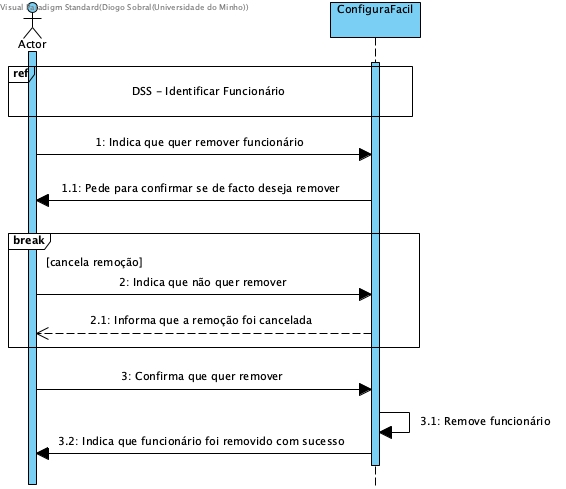
\includegraphics[width = 5.5in]{DSS/DSS-Remover_funcionario.jpg}
\end{center}

\subsection{Alterar Funcionário}
\begin{center}
 	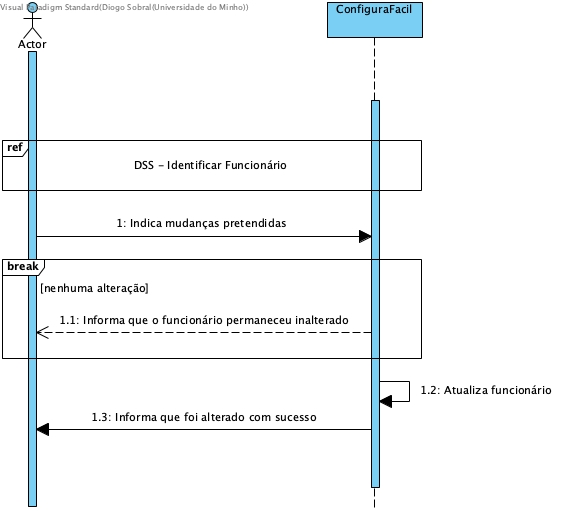
\includegraphics[width = 5.5in]{DSS/DSS-Alterar_funcionario.jpg}
\end{center}

\subsection{Identificar Cliente}
\begin{center}
 	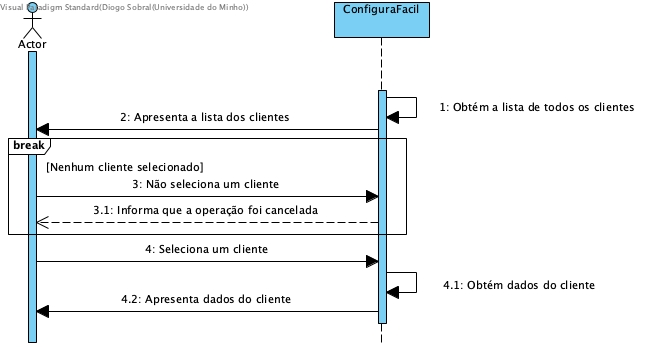
\includegraphics[width = 5.5in]{DSS/DSS-Identificar_Cliente.jpg}
\end{center}

\subsection{Alterar Cliente}
\begin{center}
 	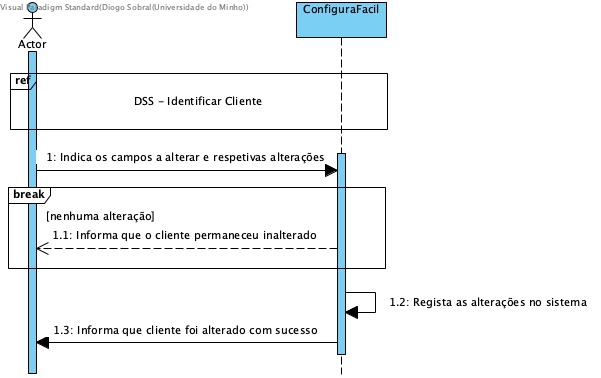
\includegraphics[width = 5.5in]{DSS/DSS-Alterar_Cliente.jpg}
\end{center}

\subsection{Registar Cliente}
\begin{center}
 	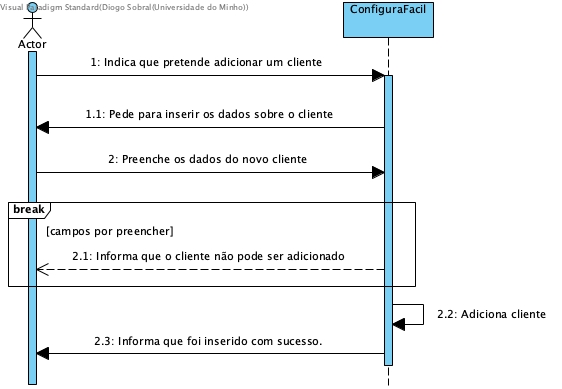
\includegraphics[width = 5.5in]{DSS/DSS-Registar_cliente.jpg}
\end{center}

\subsection{Regista Encomenda}
\begin{center}
 	\includegraphics[width = 5.5in]{DSS/DSS-Registar_Encomenda.jpg}
\end{center}

\subsection{Adicionar Componente}
\begin{center}
 	\includegraphics[width = 5.5in]{DSS/DSS-Adiciona_Componente.jpg}
\end{center}

\subsection{Adicionar pacote}
\begin{center}
 	\includegraphics[width = 5.5in]{DSS/DSS-Adiciona_Pacote.jpg}
\end{center}

\subsection{Configuração Ótima}
\begin{center}
 	\includegraphics[width = 5.5in]{DSS/DSS-Configuracao_otima.jpg}
\end{center}

\subsection{Registar Stock}
\begin{center}
 	\includegraphics[width = 5.5in]{DSS/DSS-Registar_Stock.jpg}
\end{center}

\subsection{Consultar Encomenda}
\begin{center}
 	\includegraphics[scale = 0.6]{DSS/DSS-Consultar_encomenda.jpg}
\end{center}

\subsection{Produzir Encomenda}
\begin{center}
    \centering
 	\includegraphics[scale = 0.6]{DSS/DSS-Produzir_encomenda.jpg}
\end{center}
\newpage

\section{Diagramas de Sequência com Subsistemas}
O passo seguinte foi, partindo dos diagramas de sequência e conhecendo agora os subsistemas existentes, modelar os diagramas de sequência de subsistema, para depois podemos proseguir com os diagramas de implementação.

Ora, temos então o seguinte:

\subsection{Log in}
\begin{center}
 	\includegraphics[width = 5.5in]{DSSS/DSSS-LogIn.jpg}
\end{center}

\subsection{Identificar Funcionário}
\begin{center}
 	\includegraphics[width = 5.5in]{DSSS/DSSS-Identificar_Funcionario.jpg}
\end{center}

\subsection{Registar Funcionário}
\begin{center}
 	\includegraphics[width = 5.5in]{DSSS/DSSS-Registar_Funcionario.jpg}
\end{center}

\subsection{Remover Funcionário}
\begin{center}
 	\includegraphics[width = 5.5in]{DSSS/DSSS-Remover_funcionario.jpg}
\end{center}

\subsection{Alterar Funcionário}
\begin{center}
 	\includegraphics[width = 5.5in]{DSSS/DSSS-Alterar_Funcionario.jpg}
\end{center}

\subsection{Identificar Cliente}
\begin{center}
 	\includegraphics[width = 5.5in]{DSSS/DSSS-Identificar_Cliente.jpg}
\end{center}

\subsection{Alterar Cliente}
\begin{center}
 	\includegraphics[width = 5.5in]{DSSS/DSSS-Alterar_Cliente.jpg}
\end{center}

\subsection{Registar Cliente}
\begin{center}
 	\includegraphics[width = 5.5in]{DSSS/DSSS-Registar_Cliente.jpg}
\end{center}

\subsection{Regista Encomenda}
\begin{center}
 	\includegraphics[width = 5.5in]{DSSS/DSSS-Registar_Encomenda.jpg}
\end{center}

\subsection{Adicionar Componente}
\begin{center}
 	\includegraphics[width = 5.5in]{DSSS/DSSS-Adicionar_Componente.jpg}
\end{center}

\subsection{Adicionar pacote}
\begin{center}
 	\includegraphics[width = 5.5in]{DSSS/DSSS-Adicionar_Pacote.jpg}
\end{center}

\subsection{Configuração Ótima}
\begin{center}
 	\includegraphics[width = 5.5in]{DSSS/DSSS-Configuracao_otima.jpg}
\end{center}

\subsection{Registar Stock}
\begin{center}
 	\includegraphics[width = 5.5in]{DSSS/DSSS-Registar_Stock.jpg}
\end{center}

\subsection{Consultar Encomenda}
\begin{center}
 	\includegraphics[width = 5.5in]{DSSS/DSSS-Consultar_encomenda.jpg}
\end{center}

\subsection{Produzir Encomenda}
\begin{center}
    \centering
 	\includegraphics[width = 5.5in]{DSSS/DSSS-Produzir_Encomenda.jpg}
\end{center}
\newpage

\section{Diagrama de Packages}
De forma a organizarmos melhor a aplicação, dividimos o sistema geral em quatro subsistemas: o Facade (que corresponde à ConfiguraFácil), o gContas, o gConfig e o gFabrica. Como tal, construímos o seguinte diagrama de pacotes:
\begin{center}
 	\includegraphics[width=6in]{VPP/Packages.jpg}
\end{center}
\newpage
\subsection{Camada de Negócio - Subsistemas}
\begin{itemize}
    \item \textbf{ConfiguraFácil(Facade)}\newline
    O ConfiguraFácil será responsável por produzir a ligação entre a interface gráfica e camada de negócio.
    \item \textbf{gContas} \newline
    A aplicação do stand terá de guardar e tratar informação relativa aos seus utilizadores e clientes. O gContas será o subsistema responsável por garantir que tudo isto é possível.
    \item \textbf{gConfig} \newline
    O objetivo principal da aplicação é conseguir configurar e realizar pedidos específicos por parte dos clientes. O gConfig será responsável por permitir a realização de configurações sem que estas se tornem inviáveis.
    \item \textbf{gFabrica} \newline
    A aplicação também terá capaz de gerir a produção de encomendas e garantir a existência de stock da sua fábrica. Assim, o gFabrica fica responsável pela gerência das encomendas do cliente e por gerir o stock disponível.
\end{itemize}
 %% falta ver os diagramas

\section{Diagrama de Classe com Estruturas de Dados e com ORM}
Partindo do Modelo de Domínio e dos diagramas de sequência de sistema e subsistemas, procedemos à definição do diagrama de classes, numa primeira fase, usando estruturas de dados do Java. O processo de construção foi iterativo e realizado, de certa forma, paralelamente ao desenvolvimento dos diagramas de sequência de implementação. De seguida, apresenta-se uma primeira versão do diagrama, sem implementação de persistência. Posteriormente, é apresentada a versão com DAOs. 
\begin{center}
 	\includegraphics[width=6in]{VPP/Diagrama_de_Classes.jpg}
\end{center}

\newpage
O passo seguinte foi, tendo em conta o ORM, decidir quais as classes que deveriam persistir. Assim, pela nossa análise, selecionamos as seguintes classes: Cliente, Funcionário, Encomenda, Componente, Pacote e Stock. Deste modo, obtivemos o seguinte diagrama de classes:

\begin{center}
 	\includegraphics[width=6in]{VPP/diagramadao.jpg}
\end{center}
\newpage
 %% falta ver os diagramas

\section{Diagramas de Sequência de Implementação}
Á medida que desenhamos as versões do Diagrama de Classes com e sem persistência, fomos também elaborando os diagramas de implementação dos UCs apresentados. Desta forma, conseguimos completar o Diagrama de Classes (inserindo os respetivos métodos nas classes). É de referir que o código fonte do projeto foi escrito tendo por base os diagramas de implementação. De facto, o processo de escrita foi substancialmente facilitado pelo facto dos diagramas de implementação serem bastante expressivos quanto às mensagens trocadas entre os diferentes objetos.

De seguida, apresentam-se os ditos diagramas, identificando a versão apoiada no Diagrama de Classes com estruturas de dados, e o respetivo diagrama de implementação tendo por base a versão obtida após aplicação do ORM.

\subsection{Log in}
\subsubsection{Sem DAOs}
\begin{center}
 	\includegraphics[width = 5.5in]{DSI/DSI-LogIn.jpg}
\end{center}
\subsubsection{Com DAOs}
\begin{center}
 	\includegraphics[width = 5.5in]{DSI_D/DSI-DAOs-Log_In.jpg}
\end{center}


\subsection{Identificar Funcionário}
\subsubsection{Sem DAOs}
\begin{center}
 	\includegraphics[width = 5.5in]{DSI/DSI-Identificar_Funcionario.jpg}
\end{center}
\subsubsection{Com DAOs}
\begin{center}
 	\includegraphics[width = 5.5in]{DSI_D/DSI-DAOs-Identificar_Funcionario.jpg}
\end{center}

\subsection{Registar Funcionário}
\subsubsection{Sem DAOs}
\begin{center}
 	\includegraphics[width = 5.5in]{DSI/DSI-Registar_Funcionario.jpg}
\end{center}
\subsubsection{Com DAOs}
\begin{center}
 	\includegraphics[width = 5.5in]{DSI_D/DSI-DAOs-Registar_Funcionario.jpg}
\end{center}


\subsection{Remover Funcionário}
\subsubsection{Sem DAOs}
\begin{center}
 	\includegraphics[width = 5.5in]{DSI/DSI-Remover_Funcionario.jpg}
\end{center}
\subsubsection{Com DAOs}
\begin{center}
 	\includegraphics[width = 5.5in]{DSI_D/DSI-DAOs-Remover_Funcionario.jpg}
\end{center}


\subsection{Alterar Funcionário}
\subsubsection{Sem DAOs}
\begin{center}
 	\includegraphics[width = 5.5in]{DSI/DSI-Alterar_Funcionario.jpg}
\end{center}
\subsubsection{Com DAOs}
\begin{center}
 	\includegraphics[width = 5.5in]{DSI_D/DSI-DAOs-Alterar_Funcionario.jpg}
\end{center}


\subsection{Identificar Cliente}
\subsubsection{Sem DAOs}
\begin{center}
 	\includegraphics[width = 5.5in]{DSI/DSI-Identificar_Cliente.jpg}
\end{center}
\subsubsection{Com DAOs}
\begin{center}
 	\includegraphics[width = 5.5in]{DSI_D/DSI-DAOs-Identificar_Cliente.jpg}
\end{center}


\subsection{Alterar Cliente}
\subsubsection{Sem DAOs}
\begin{center}
 	\includegraphics[width = 5.5in]{DSI/DSI-Alterar_Cliente.jpg}
\end{center}
\subsubsection{Com DAOs}
\begin{center}
 	\includegraphics[width = 5.5in]{DSI_D/DSI-DAOs-Alterar_Cliente.jpg}
\end{center}


\subsection{Registar Cliente}
\subsubsection{Sem DAOs}
\begin{center}
 	\includegraphics[width = 5.5in]{DSI/DSI-Registar_Cliente.jpg}
\end{center}
\subsubsection{Com DAOs}
\begin{center}
 	\includegraphics[width = 5.5in]{DSI_D/DSI-DAOs-Registar_Cliente.jpg}
\end{center}

\subsection{Regista Encomenda}
\subsubsection{Sem DAOs}
\begin{center}
 	\includegraphics[width = 5.5in]{DSI/DSI-Registar_Encomenda.jpg}
\end{center}
\subsubsection{Com DAOs}
\begin{center}
 	\includegraphics[width = 5.5in]{DSI_D/DSI-DAOs-Registar_Encomenda.jpg}
\end{center}


\subsection{Adicionar Componente}
\subsubsection{Sem DAOs}
\begin{center}
 	\includegraphics[width = 5.5in]{DSI/DSI-Adicionar_Componente.jpg}
\end{center}
\subsubsection{Com DAOs}
\begin{center}
 	\includegraphics[width = 5.5in]{DSI_D/DSI-c_DAOs-Adicionar_Componente.jpg}
\end{center}


\subsection{Adicionar pacote}
\subsubsection{Sem DAOs}
\begin{center}
 	\includegraphics[width = 5.5in]{DSI/DSI-Adicionar_Pacote.jpg}
\end{center}
\subsubsection{Com DAOs}
\begin{center}
 	\includegraphics[width = 5.5in]{DSI_D/DSI-DAOs-Adicionar_Pacote.jpg}
\end{center}


\subsection{Configuração Ótima}
\subsubsection{Sem DAOs}
\begin{center}
 	\includegraphics[width = 5.5in]{DSI/DSI-Configuracao_Otima.jpg}
\end{center}
\subsubsection{Com DAOs}
\begin{center}
 	\includegraphics[width = 5.5in]{DSI_D/DSI-DAOs-Configuracao_Otima.jpg}
\end{center}


\subsection{Registar Stock}
\subsubsection{Sem DAOs}
\begin{center}
 	\includegraphics[width = 5.5in]{DSI/DSI-Registar_Stock.jpg}
\end{center}
\subsubsection{Com DAOs}
\begin{center}
 	\includegraphics[width = 5.5in]{DSI_D/DSI-DAOs-Registar_Stock.jpg}
\end{center}


\subsection{Consultar Encomenda}
\subsubsection{Sem DAOs}
\begin{center}
 	\includegraphics[width = 5.5in]{DSI/DSI-Consultar_Encomenda.jpg}
\end{center}
\subsubsection{Com DAOs}
\begin{center}
 	\includegraphics[width = 5.5in]{DSI_D/DSI-DAOs-Consultar_Encomenda.jpg}
\end{center}


\subsection{Produzir Encomenda}
\subsubsection{Sem DAOs}
\begin{center}
 	\includegraphics[width = 5.5in]{DSI/DSI-Produzir_Encomenda.jpg}
\end{center}
\subsubsection{Com DAOs}
\begin{center}
 	\includegraphics[width = 5.5in]{DSI_D/DSI-DAOs-Produzir_Encomenda.jpg}
\end{center}
\newpage


\section{Implementação}
Antes de começarmos a implementar a aplicação, decidimos estabelecer primeiro os dados do programa, isto é, os componentes e pacotes existentes, bem como as incompatibilidades e complementaridades entre si.

No que toca a componentes, dividimo-los em seis tipos, com as seguintes especificações:
\begin{enumerate}
    \item Pintura \begin{itemize} \item Cinzento \item Branco \item Preto \end{itemize}
    \item Jantes \begin{itemize} \item 19" \item 20" \item 21" \end{itemize}
    \item Pneus \begin{itemize} \item Normal \item Largo \item XL \item Off-road \end{itemize}
    \item Motorização \begin{itemize} \item 1.0 \item 1.4 \item 1.6 \item 1.8 \item 2.0 \item Turbo \end{itemize}
    \item Vidros \begin{itemize} \item Normais \item Escurecidos \end{itemize}
    \item Estofos \begin{itemize} \item Tecido - Cinzentos \item Tecido - Pretos \item Pele - Castanhos \item Pele - Pretos \end{itemize}
\end{enumerate}

Relativamente às relações, definimos que todos os componentes dum mesmo tipo são incompatíveis entre si. Além dessas incompatibilidades, escolhemos incompatibilizar as jantes 19" com os pneus XL e Off-road, bem como a motorização Turbo com as jantes 19" e os pneus Normais. Porém, existem também relações de complementaridade, como foi referido anteriormente. Estas dizem respeito ao seguinte: a jante 19" precisa de um pneu Normal, o pneu XL precisa de uma jante 20", o pneu Off-road precisa de uma jante 21" e a motorização Turbo necessita de um pneu XL.

No que toca aos pacotes, definimos também seis: o \textit{Sport}, o \textit{Comfort}, \textit{Off-road}, \textit{Executive}, \textit{Classic} e \textit{Economic}.

Os componentes englobados em cada pacote são os seguintes:
\begin{enumerate}
    \item \textit{Sport}: Jantes 20", Pneus XL, Motorização Turbo e Estodos de Tecido Pretos
    \item \textit{Comfort}: Pintura Cinzenta, Pneus Largos e Estofos de Tecido Cinzentos
    \item \textit{Off-road}: Jantes 21", Pneus Off-road e Motorização 2.0
    \item \textit{Executive}: Pintura Preta, Motorização 1.8, Vidros Escurecidos e Estofos de Pele Pretos
    \item \textit{Classic}: Pintura Branca, Jantes 19", Motorização 1.0 e Estofos de Pele Castanhos
    \item \textit{Economic}: Jantes 20" e Motorização 1.4.
\end{enumerate}


\subsection{Algoritmo de Configuração ótima}
Uma das funcionalidades propostas permite o calculo automático de uma configuração quando dado um orçamento. O nosso algoritmo para o calculo da mesma é descrito da seguinte maneira:
\begin{enumerate}
    \item Usando uma lista com todos os componentes, construimos a lista prim com apenas os componentes com dependências e a lista sng com componentes sem dependências.
    \item Ordenamos a lista prim pela razão entre o custo total (custo componente + custo das dependências) e o número de componentes que são adicionados. (heuristica da razão)
    \item Ordenamos a lista sng pelo custo.
    \item Iteramos a lista prim e adicionamos o componente à configuração se for possível adicionar todas as suas dependências sem que o orçamento seja ultrapassado ou que a configuração tenha incompatibilidades.
    \item Por fim iteramos a lista sng e, se for possível, adicionamos o componente à configuração.
\end{enumerate}

Este algoritmo construi uma configuração válida e dentro do orçamento.

\newpage
\subsection{Base de dados implementada}
Ao transformar o diagrama de classes num diagrama com ORM foi necessário que algumas classes passassem a persistir e, para tal, implementamos um sistema de dados MySQL. De seguida é apresentado o modelo lógica do mesmo:

\begin{center}
 	\includegraphics[width = 5.5in]{VPP/modelologico.png}
\end{center}
\newpage

\section{Interface}

Nesta secção é explicada a interface da aplicação, ou seja, o \textit{flow} entre as várias janelas, assim como o que o utilizador pode fazer nestas e a forma para tal.

\subsection{Login}
Iniciando a aplicação, o utilizador fica perante a janela de \textit{login}, apresentada na Figura \ref{loginframe}. 
\begin{figure}[H]
	\centering
	\includegraphics[]{loginframe.png}
	\caption{Login Frame}
	\label{loginframe}
\end{figure}

Para o efetuar, é necessário, antes de tudo, estar registado no sistema e, para tal, apenas o administrador (com conta predefinida) o poderá fazer.

Nesta janela, e conforme o tipo de funcionário que esteja a realizar o login, a próxima janela é uma das seguintes:
\begin{itemize}
	\item Stand (ver Secção \ref{standsec})
	\item Fábrica (ver Secção \ref{fabricasec})
	\item Gestão de funcionários (ver Secção \ref{adminsec})
\end{itemize}

\subsection{Stand}
\label{standsec}

Iniciando sessão como \textit{Funcionário de loja}, a janela correspondente é a apresentada na Figura \ref{standframe}.
\begin{figure}[H]
	\centering
	\includegraphics[]{standframe.png}
	\caption{Stand Frame}
	\label{standframe}
\end{figure}

A partir daqui o utilizador pode iniciar uma configuração, consultar todos os clientes registados no sistema ou fazer \textit{logout} através dos botões \textit{"Iniciar Configuração"}, \textit{"Consultar Clientes"} e \textit{"Sair"}, respetivamente. Nesta janela, é também possível ver o utilizador que está com sessão iniciada no canto inferior direito.

\subsubsection{Configuração}
Na criação de uma configuração podem ser adicionadas componentes ou pacotes de componentes.

\begin{figure}[H]
	\centering
	\includegraphics[]{configframe.png}
	\caption{Configuração Frame}
	\label{configframe}
\end{figure}

Para adicionar uma componente é preciso, primeiro, escolher o seu tipo e, só depois, é que se torna possível selecioná-la. Para a escolha de um pacote, é possível visualizar o seu conteúdo primeiro clicando no pacote desejado. O pacote apenas fica selecionado quando é feito \textit{double click} sobre o mesmo (aparecendo um visto no pacote). Tal comportamento pode ser visualizado na Figura \ref{configframe}.
Neste processo de adicionar componentes podem surgir casos em que a componente desejada cria incompatibilidades com uma ou mais componentes já existentes na configuração ou, então, a componente a adicionar ter componentes que são complementares e necessitam também de ser adicionadas. A resolução destes problemas é resolvida conforme as figuras abaixo:

\begin{figure}[H]
	\centering
	\includegraphics[]{incompativeis.png}
\end{figure}

\begin{figure}[H]
	\centering
	\includegraphics[]{complementares.png}
\end{figure}




\myparagraph{Encomenda}

Neste janela (Figura \ref{regencomendaframe}), é possível para o funcionário selecionar o cliente que está a realizar a configuração, assim como verificar todas as componentes presentes na configuração, o total do preço individual das componentes, o desconto total originado pelos pacotes e o preço final da encomenda. Caso o cliente não exista no sistema, é ainda possível criá-lo a partir desta janela (processo de criação explicado na Secção \ref{novocliente}). Após selecionar o cliente e verificar as componentes, é necessário registar a encomenda clicando em \textit{Registar Encomenda}.

\begin{figure}[H]
	\centering
	\includegraphics[]{regencomendaframe.png}
	\caption{Encomenda Frame}
	\label{regencomendaframe}
\end{figure}

Caso o funcionário não selecione um cliente ou clique no botão \textit{"Sair"}, são mostradas as seguintes mensagens de erro, respetivamente:

\begin{figure}[H]
	\centering
	\includegraphics[]{erroencomenda.png}
	\caption{Erro - Cliente não selecionado}
	\label{erroencomenda}
\end{figure}

\begin{figure}[H]
	\centering
	\includegraphics[]{erroencomenda2.png}
	\caption{Erro - Não confirma encomenda}
	\label{erroencomenda2}
\end{figure}



\subsubsection{Consultar clientes}
Para além da funcionalidade descrita na secção anterior, o \textit{Funcionário de loja} pode ainda, na janela apresentada na Figura \ref{clientesframe}, consultar, pesquisar e alterar clientes, assim como adicionar novos. 

Na tabela estão presentes os clientes registados no sistema até ao momento. Estes podem ser pesquisados pelo seu nome, utilizando para tal a caixa de texto presente debaixo da tabela. Ao fazer \textit{double click} sobre um cliente, é possível ver as suas características, bem como editar algumas delas (este processo é detalhado na secção \ref{alterarcliente}). Por fim, a partir desta janela é ainda possível a criação de novos clientes através do botão \textit{"Adicionar Cliente"} (como é demonstrado na secção \ref{novocliente}).

\begin{figure}[H]
	\centering
	\includegraphics[]{clientesframe.png}
	\caption{Clientes Frame}
	\label{clientesframe}
\end{figure}


\myparagraph{Novo Cliente}
\label{novocliente} 

Para registar um novo cliente é necessário introduzir o seu nome, telemóvel e e-mail nas respestivas caixas de texto apresentadas na Figura \ref{novoclienteframe}.

\begin{figure}[H]
	\centering
	\includegraphics[]{novoclienteframe.png}
	\caption{Novo Cliente Frame}
	\label{novoclienteframe}
\end{figure}


\myparagraph{Alterar Cliente}
\label{alterarcliente}

Em relação à alteração de um cliente, apenas é permitido alterar o seu telemóvel e o seu e-mail. Para isso, é necessário que sejam feitas alterações nos respetivos campos, confirmando-as clicando em \textit{"Atualizar"}.

\begin{figure}[H]
	\centering
	\includegraphics[]{alterarclienteframe.png}
	\caption{Alterar Cliente Frame}
	\label{alterarclienteframe}
\end{figure}


\subsection{Fábrica}
\label{fabricasec}

Quando a sessão é iniciada por um \textit{Gestor de Fábrica}, a janela correspondente é a seguinte:

\begin{figure}[H]
	\centering
	\includegraphics[]{fabricaframe.png}
	\caption{Fabrica Frame}
	\label{fabricaframe}
\end{figure}

Aqui, o funcionário pode visualizar as encomendas pendentes ou atualizar o stock da fábrica. Para isso, basta clicar nos botões \textit{"Visualizar Encomendas"} e \textit{"Atualizar Stock"}, respetivamente.

\subsubsection{Encomendas Pendentes}
A partir desta janela, o funcionário pode visualizar todas as encomendas pendentes. Além do mais, é ainda possível visualizar o seu conteúdo, selecionando a desejada e em seguida clicar em \textit{Consultar} ou então produzir, no botão \textit{"Produzir Encomenda}.

\begin{figure}[H]
	\centering
	\includegraphics[]{encomendasframe.png}
	\caption{Encomendas Frame}
	\label{encomendasframe}
\end{figure}


\myparagraph{Consultar Encomenda}

Na Figura \ref{dencomendasframe}, é apresentado um exemplo dos detalhes de uma encomenda:

\begin{figure}[H]
	\centering
	\includegraphics[]{detalhesencomenda.png}
	\caption{Detalhes Encomenda Frame}
	\label{dencomendasframe}
\end{figure}

\myparagraph{Produzir Encomenda}

Para que seja possível produzir uma encomenda, é necessário que exista stock de todas as componentes presentes na mesma. Uma possível mensagem é a seguinte:

\begin{figure}[H]
	\centering
	\includegraphics[]{stockinsuficiente.png}
\end{figure}

O utilizador ao responder "sim" são-lhe apresentadas, então, as componentes sem stock de momento:

\begin{figure}[H]
	\centering
	\includegraphics[]{componentesemfalta.png}
\end{figure}

\subsubsection{Stock}
Como se pode ver pela Figura \ref{stockframe}, nesta janela é apresentado todo o stock das componentes existentes (ordenado por ordem decrescente de stock). Para atualizar stock é necessário clicar em \textit{"Atualizar Stock"}. Esse processo é explicado na secção seguinte.

\begin{figure}[H]
	\centering
	\includegraphics[]{stockframe.png}
	\caption{Stock Frame}
	\label{stockframe}
\end{figure}

\myparagraph{Atualizar Stock}

Quando o funcionário necessita de atualizar stock é confrontado com a seguinte janela:
\begin{figure}[H]
	\centering
	\includegraphics[]{encomendastock1.png}
\end{figure}

Caso o ID da componente introduzido exista prossegue introduzindo a quantidade:

\begin{figure}[H]
	\centering
	\includegraphics[]{encomendastock2.png}
\end{figure}

Caso não exista a componente o funcionário é interrogado se quer ou não adicionar nova componente:
\begin{figure}[H]
	\centering
	\includegraphics[]{adicionarcomp.png}
\end{figure}

Se não aceitar adicionar o processo para. Se adicionar tem então que introduzir as características da nova componente:
\begin{figure}[H]
	\centering
	\includegraphics[width=5in]{novacomponente.png}
\end{figure}

Aqui é possível também adicionar componentes complementares ou incompatíveis caso existam algumas sem nenhum destes dois inconvenientes. Para finalizar este registo apenas tem que clicar em \textit{"Adicionar"}.


\subsection{Gestão de funcionários}
\label{adminsec}

Por fim, o último caso de login é quando ele é realizado pelo administrador. A partir da janela identificada na Figura \ref{funcionariosframe}, este é capaz de adicionar novos funcionários e gerir os já existentes. Para a primeira funcionalidade, o utilizador necessita de clicar no botão \textit{"Adicionar funcionário"} enquanto que para a segunda é necessário fazer \textit{double click} no funcionário desejado. Estas funcionalidades são explicadas mais detalhadamente nas secções em seguida (\ref{novofunc} e \ref{alterafunc}, respetivamente). É também possível para o utilizador pesquisar por um funcionário através da caixa de texto presente na janela. A tabela dos funcionários é atualizada conforme o que é introduzido nessa caixa.


\begin{figure}[H]
	\centering
	\includegraphics[]{funcionariosframe.png}
	\caption{Funcionarios Frame}
	\label{funcionariosframe}
\end{figure}

\subsubsection{Novo funcionário}
\label{novofunc}

Para a criação de um novo funcionário é necessário preencher todos os campos presentes na Figura \ref{novofuncframe}. O tipo do funcionário pode variar entre \textit{"1 - Funcionário de loja"} e \textit{"2 - Gestor de fábrica"}.

\begin{figure}[H]
	\centering
	\includegraphics[]{novofuncframe.png}
	\caption{Novo Funcionário Frame}
	\label{novofuncframe}
\end{figure}


\subsubsection{Alterar funcionário}
\label{alterafunc}

Nesta janela, e para concluir a interface, é possível, como referido anteriormente, gerir o funcionário selecionado. Esta gestão pode ser a alteração dos seus dados (exceto \textit{nome} e \textit{password}) ou a sua remoção do sistema.

\begin{figure}[H]
	\centering
	\includegraphics[]{alterarfuncframe.png}
	\caption{Alterar Funcionário Frame}
	\label{alterarfuncframe}
\end{figure}
\newpage

\section{Análise Crítica}
Na primeira fase do trabalho pediram-nos para fazer uma análise mais abstrata de modo a criar uma primeira imagem e ideia sobre a aplicação que estamos a desenvolver. A nossa abordagem começou pelo desenvolvimento do modelo domínio. Aqui tentamos estabelecer as principais entidades e as relações entre as mesmas de modo a criar a nossa primeira interpretação sobre o problema. Inicialmente, deparámo-nos com alguns erros de interpretação do enunciado como a função do cliente na aplicação que inicialmente achávamos que ia ser o principal utilizador e mais tarde foi alterado. Esta parte da modulação fez como que a nossa visão sobre o que queríamos para a aplicação ficasse mais clara e expressa de uma forma mais simplista. Ao modelo de domínio seguiu-se o desenvolvimento dos Use Case. Quando começamos o desenvolvimento dos mesmos, focámo-nos essencialmente em descrever a ação entre os atores e a aplicação. Esta descrição foi demasiado detalhada, fornecia informação que não era precisa e sobretudo limitava muito aquilo que queríamos fazer da aplicação. Como ainda nos encontrávamos numa fase inicial decidimos refletir melhor sobre a nossa solução e chegamos à conclusão que eram limitações que não queríamos ter. A isto seguiu-se uma reestruturação do problema de uma forma mais genérica que descrevia, na mesma, todas as funcionalidades dando-nos uma margem maior para aquilo que pode vir a ser a nossa aplicação.
Seguidamente demos inicio ao desenvolvimento das máquinas de estado. Aqui tentamos recriar os diversos estados da nossa aplicação e entender como é que estes alternavam entre si. O nosso principal obstáculo foi a dificuldade em exprimir os estados durante a personalização de uma configuração, no entanto após ter sido ultrapassada facilitou a forma como iríamos desenvolver o prototipo da interface gráfica e levou-nos a uma melhor compreensão sobre a implementação das diversas funcionalidades. Por fim, chegou a altura de desenhar o primeiro prototipo. Focámo-nos essencialmente em conseguir arranjar maneiras de implementar todas as nossas funcionalidades que tínhamos previstas seguindo os nossos Use Cases. De um modo geral, esta modelação ajudou-nos a prever futuros problemas e contribuiu para conseguir formular aquilo que queremos para o futuro da aplicação.

No que diz respeito à segunda parte do trabalho, podemos concluir que foi bastante mais trabalhosa, uma vez que tivemos que definir todos os diagramas de sequência de sistema e os de subsistema. Posteriormente, tivemos ainda que modelar os de implementação, que se tornaram bastante complexos e de difícil idealização. Partindo do modelo de domínio e dos modelos de sistema e implementação, pudemos definir o diagrama de classes, o qual, à medida que íamos desenhando os de implementação, fomos atualizando o diagrama de classes com os métodos e atributos respetivos a cada classe. Aquando da inicialização da implementação, seguindo os diagramas, foi um processo muito menos dispendioso, pois possuíamos já uma base fundamentada e estruturada para cada um dos requisitos que queríamos implementar, sendo os Use Cases a base com que trabalhamos. Porém, após termos implementado a UI e apesar desta cumprir os requisitos, reparamos que algumas interação não correspondiam ao descrito nos Use Cases anteriormente definidos, pelo que tivemos que alterar a interação do sistema com o utilizador, de modo a ser realizada como tinha sido idealizada e modelada. Em suma, a modelação do programa realizada por etapas nas fases precedentes à implementação, apesar de ter sido bastante dispendiosa e elaborada, permitiu-nos poupar tempo na construção física do sistema em si, permitindo-nos que este apresentasse menos erros (sendo estes apenas relativos à codificação das interações da UI).

Em suma, a aplicação por nós construída foi, na opinião do grupo, muito bem conseguida, pois, além de ser apelativa e de fácil utilização, respeita e cumpre todos os requisitos propostos no enunciado do trabalho, bem no início do projeto. Os modelos requeridos foram todos apresentados da forma mais correta que conseguimos, e foram utilizados como pilares para a implementação da aplicação em si. Estamos, portanto, perante um sistema totalmente utilizável no mundo real, e que poderia facilitar a configuração personalizada de um carro novo.

\end{document}
